% TODO Anhänge anfügen
% Wir haben dies jeweils über \chapter gelöst
% \includepdf[pages=-]{PDF-ANHANG}
\chapter{Supplementary Material}
\label{ch:Supplementary}


\begin{figure*}
    \centering
    \setlength{\tabcolsep}{1pt}
    \Large
    \resizebox{\textwidth}{!}{%
        \begin{tabular}{C{5em}ccccc}
            & Level 1 & Level 2 & Level 3 & Level 4 & Level 5 \\
            Brighten & 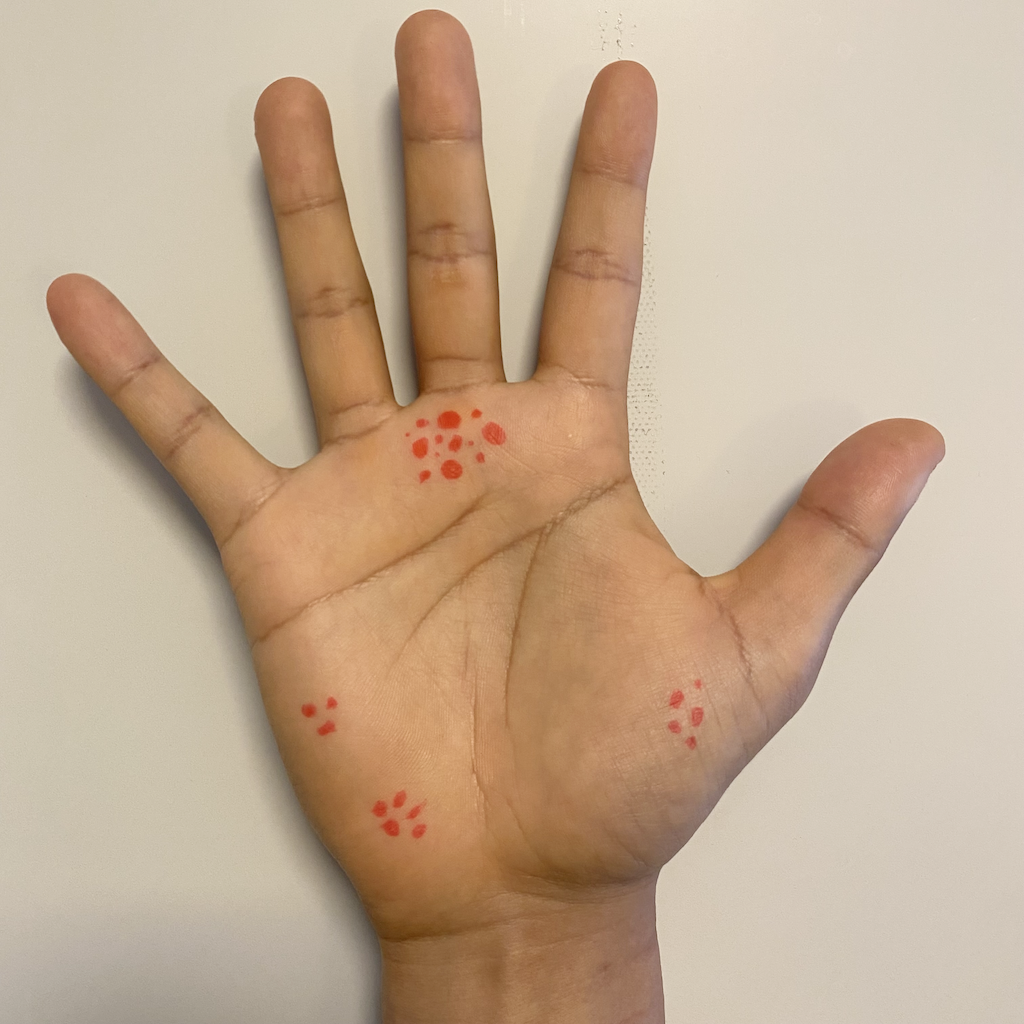
\includegraphics[width=\gridimagewidth,valign=m]{img/supplementary/lighting/brighten/0_brighten_0.0.png} & 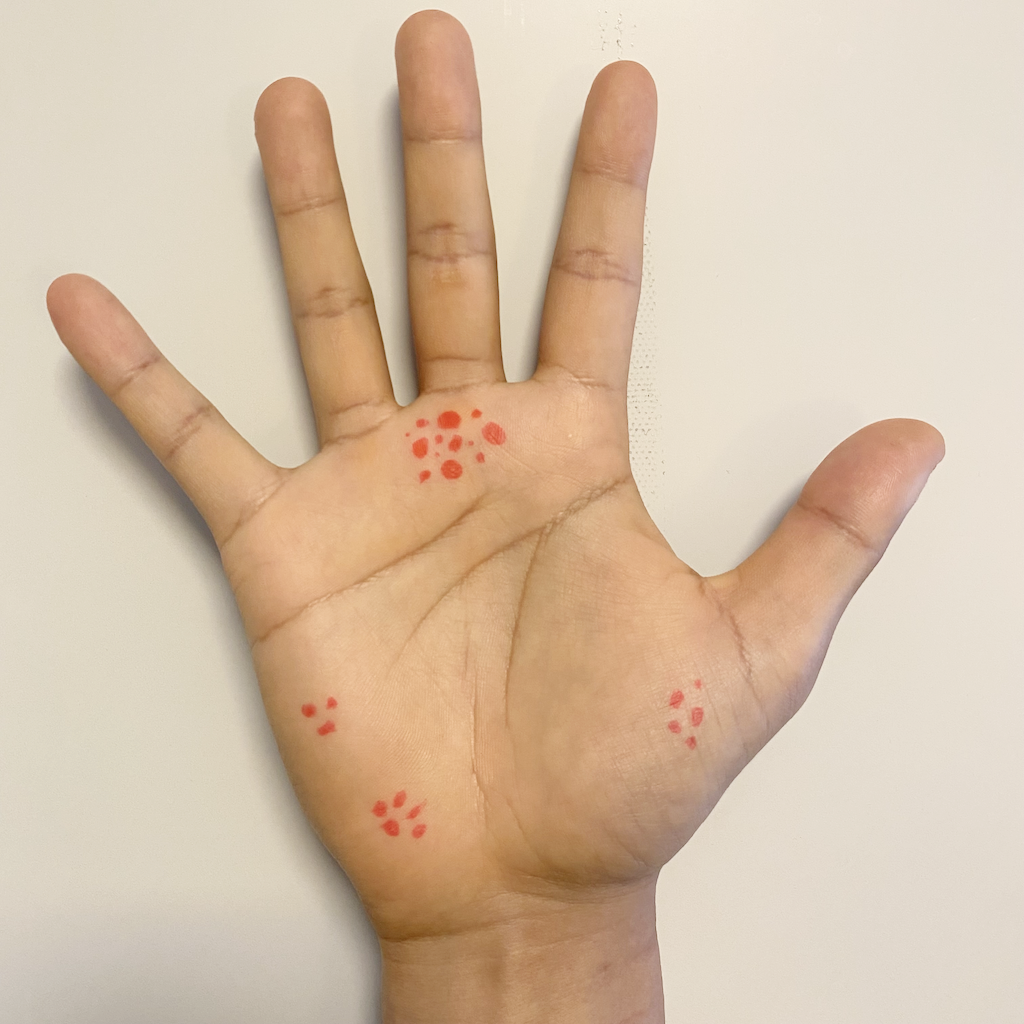
\includegraphics[width=\gridimagewidth,valign=m]{img/supplementary/lighting/brighten/0_brighten_0.2.png} & 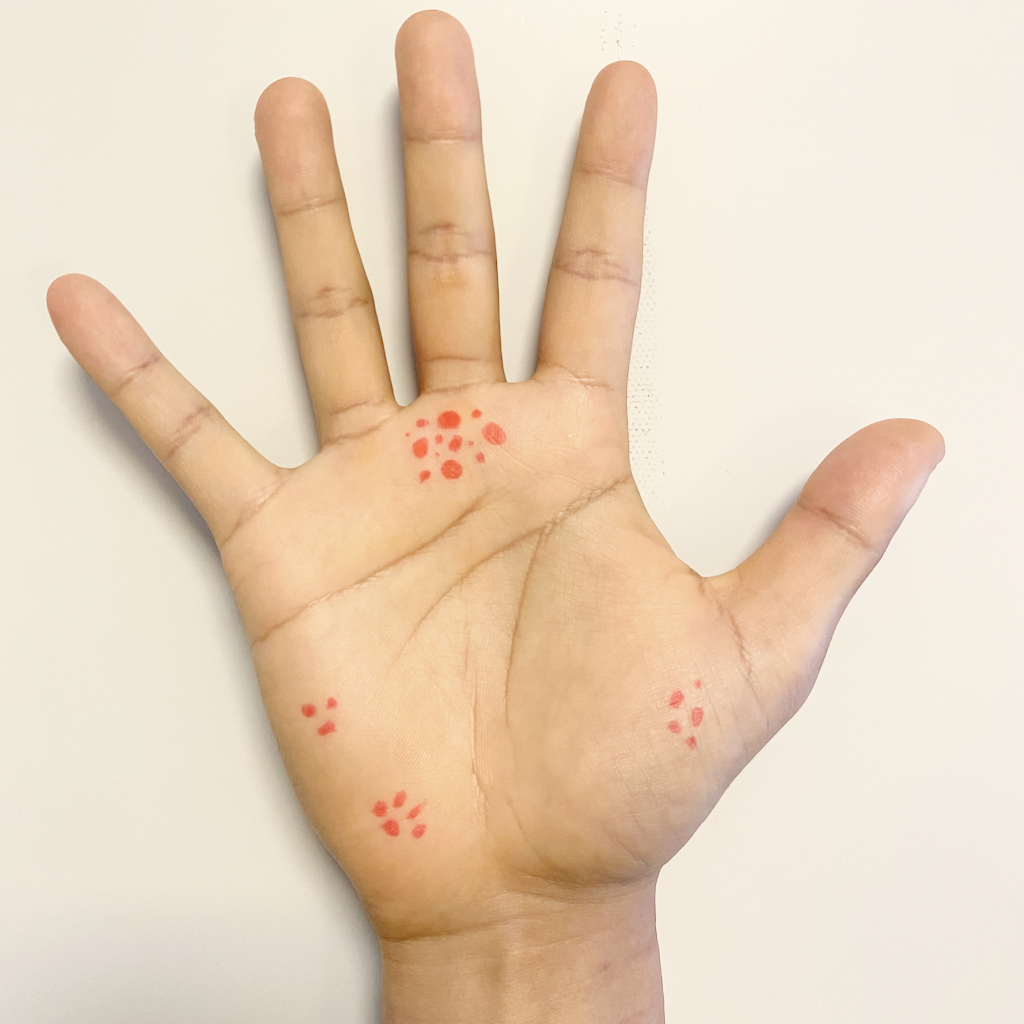
\includegraphics[width=\gridimagewidth,valign=m]{img/supplementary/lighting/brighten/0_brighten_0.4.png} & 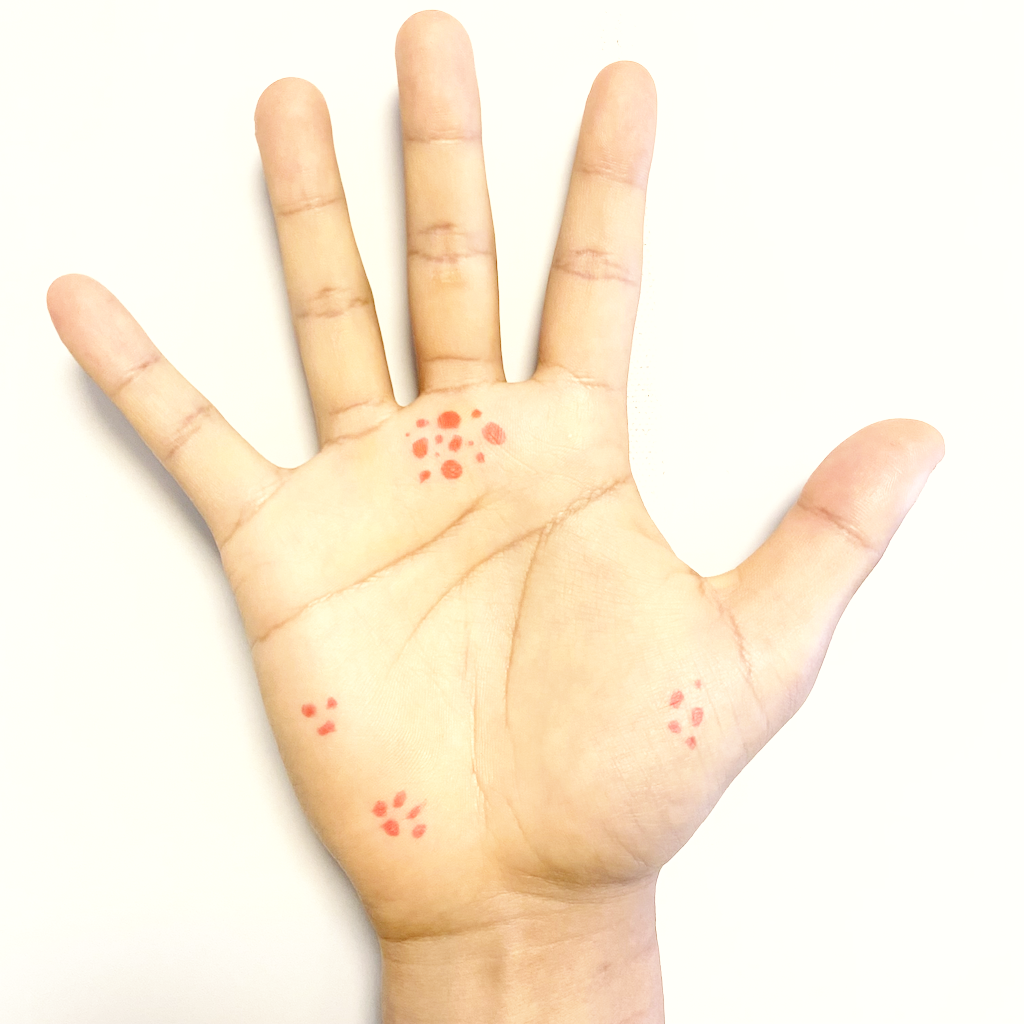
\includegraphics[width=\gridimagewidth,valign=m]{img/supplementary/lighting/brighten/0_brighten_0.7.png} & 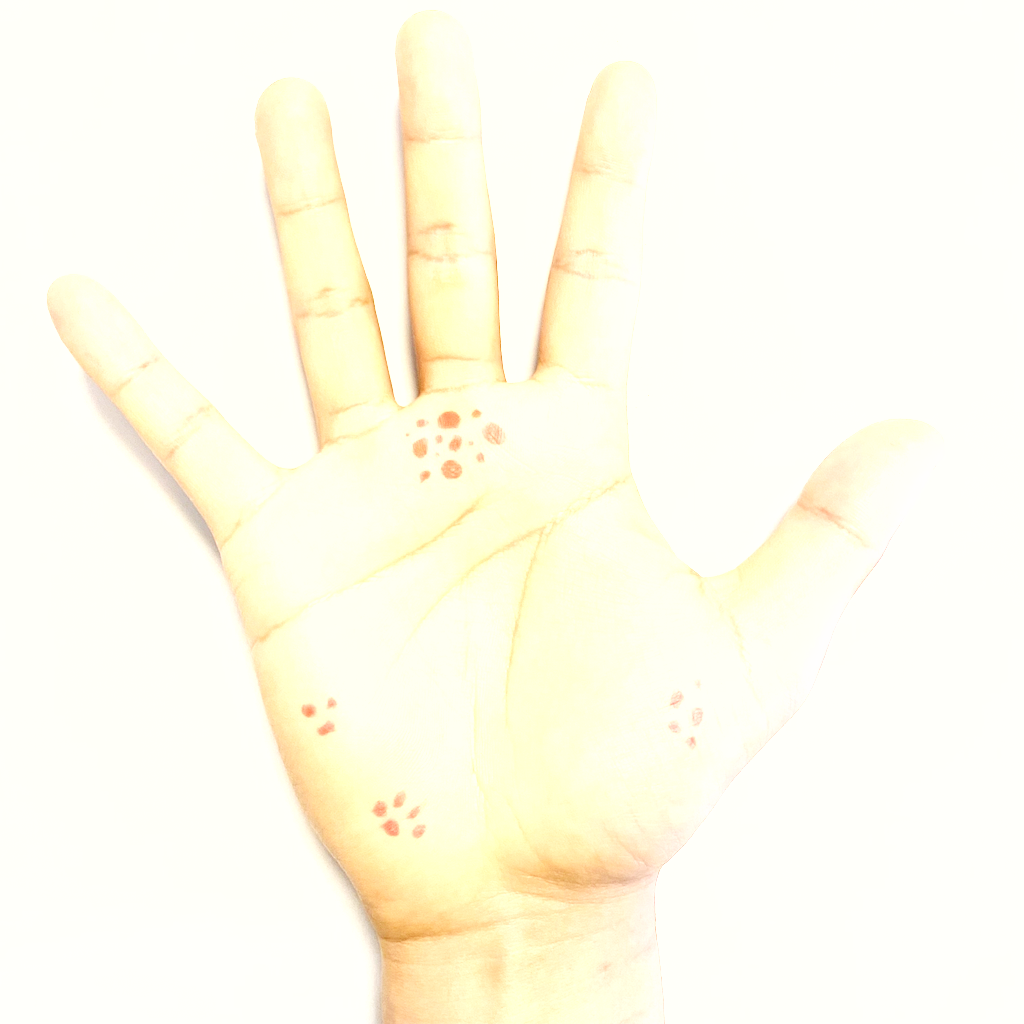
\includegraphics[width=\gridimagewidth,valign=m]{img/supplementary/lighting/brighten/0_brighten_1.1.png} \\ [6.15ex]
            Darken & 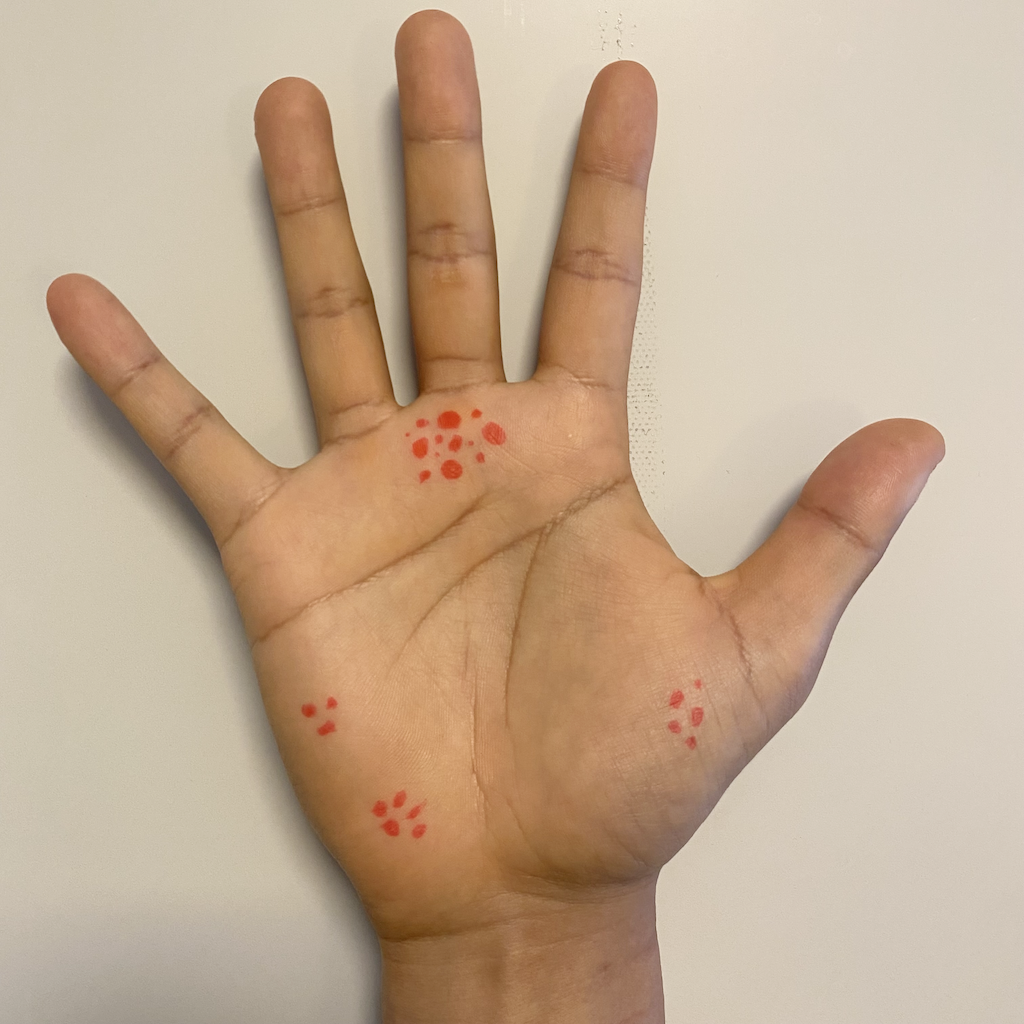
\includegraphics[width=\gridimagewidth,valign=m]{img/supplementary/lighting/darken/0_darken_0.0.png} & 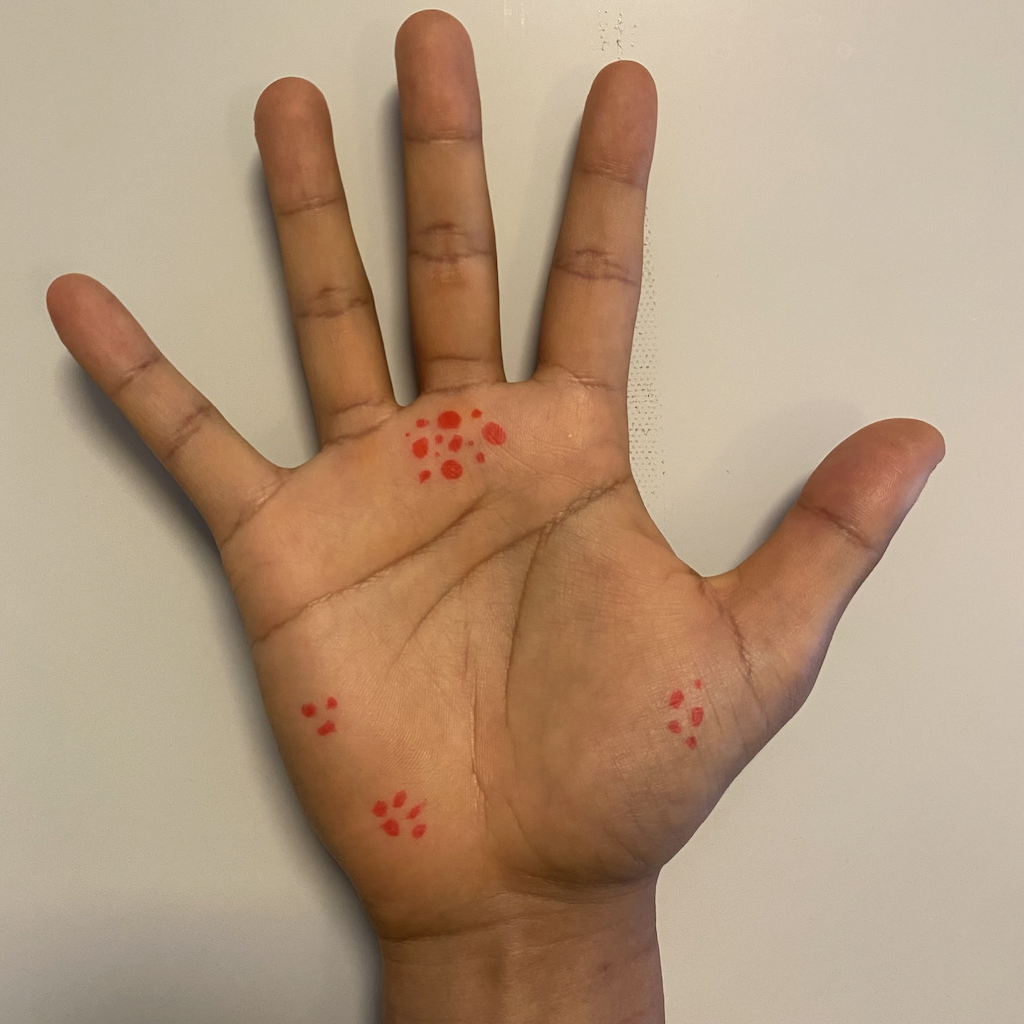
\includegraphics[width=\gridimagewidth,valign=m]{img/supplementary/lighting/darken/0_darken_0.2.png} & 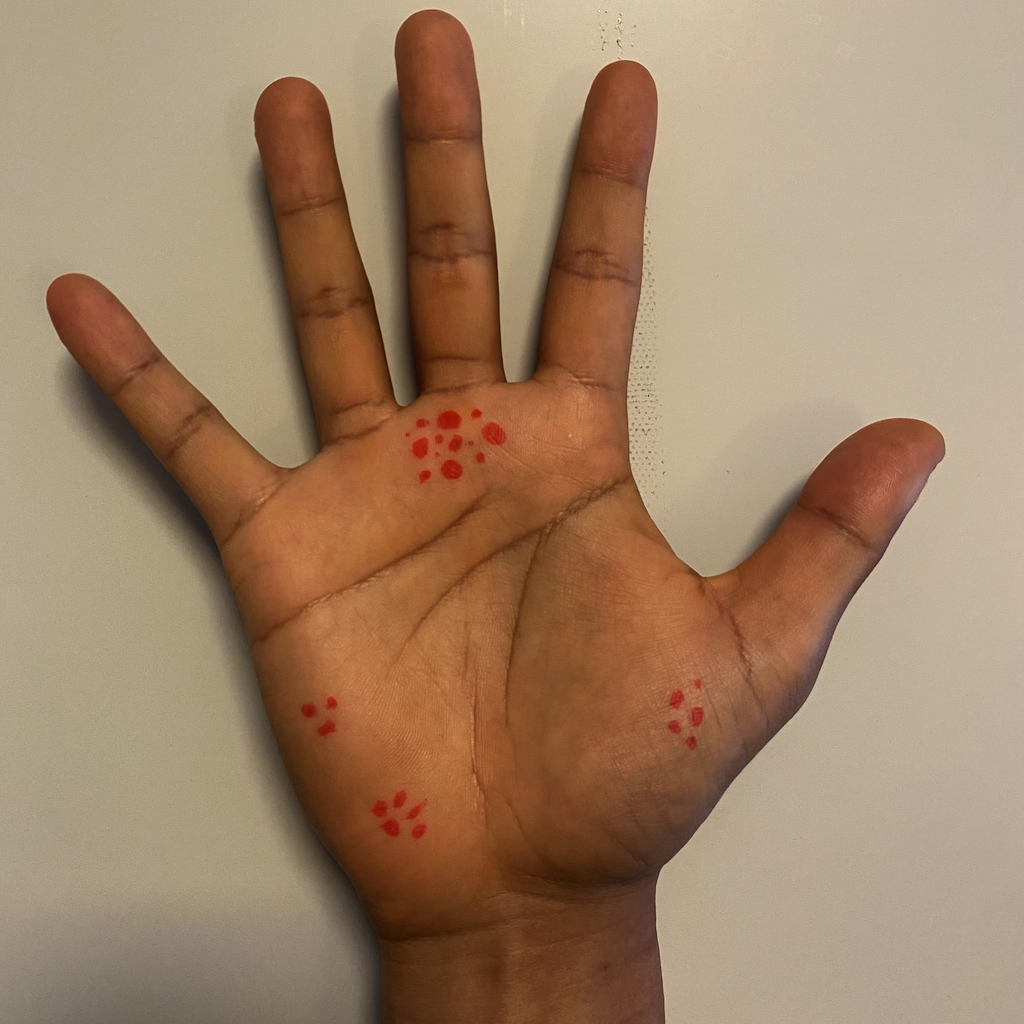
\includegraphics[width=\gridimagewidth,valign=m]{img/supplementary/lighting/darken/0_darken_0.4.png} & 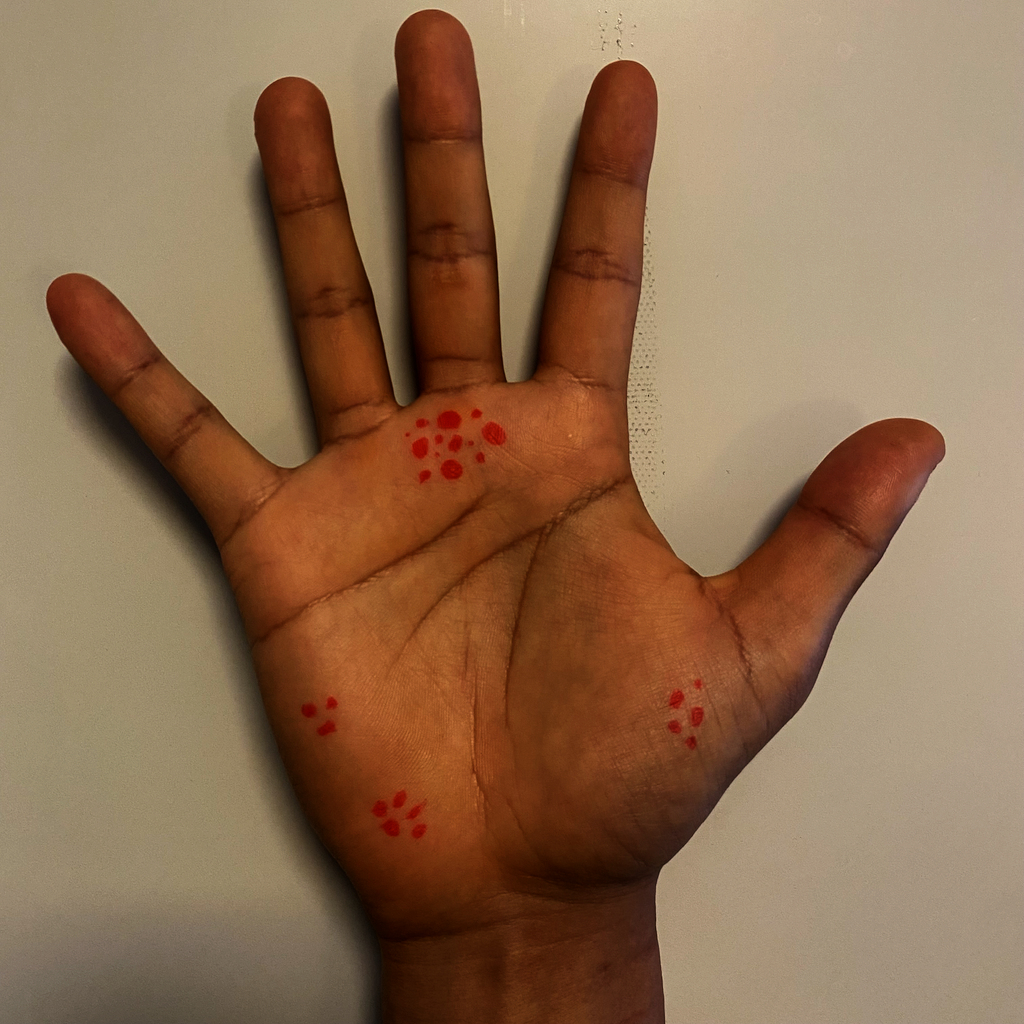
\includegraphics[width=\gridimagewidth,valign=m]{img/supplementary/lighting/darken/0_darken_0.6.png} & 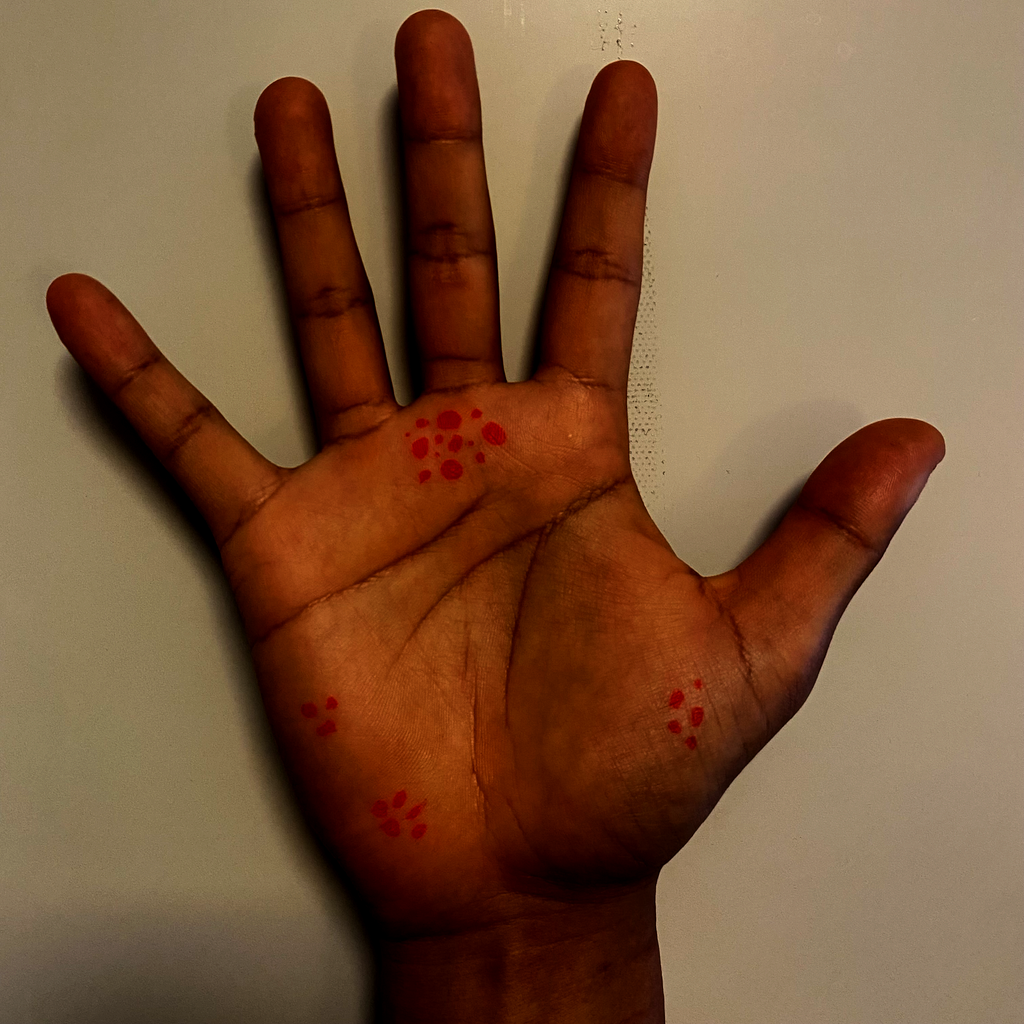
\includegraphics[width=\gridimagewidth,valign=m]{img/supplementary/lighting/darken/0_darken_0.8.png} \\ [6.15ex]
        \end{tabular}
    }
    \caption{Visualization of the degradation types belonging to the \textit{Brightness change} group for increasing levels of intensity.}
    \label{fig:brightness_change_supplementary}
\end{figure*}

\begin{figure*}
    \centering
    \setlength{\tabcolsep}{1pt}
    \Large
    \resizebox{\textwidth}{!}{%
        \begin{tabular}{C{5em}ccccc}
            & Level 1 & Level 2 & Level 3 & Level 4 & Level 5 \\
            Color block & 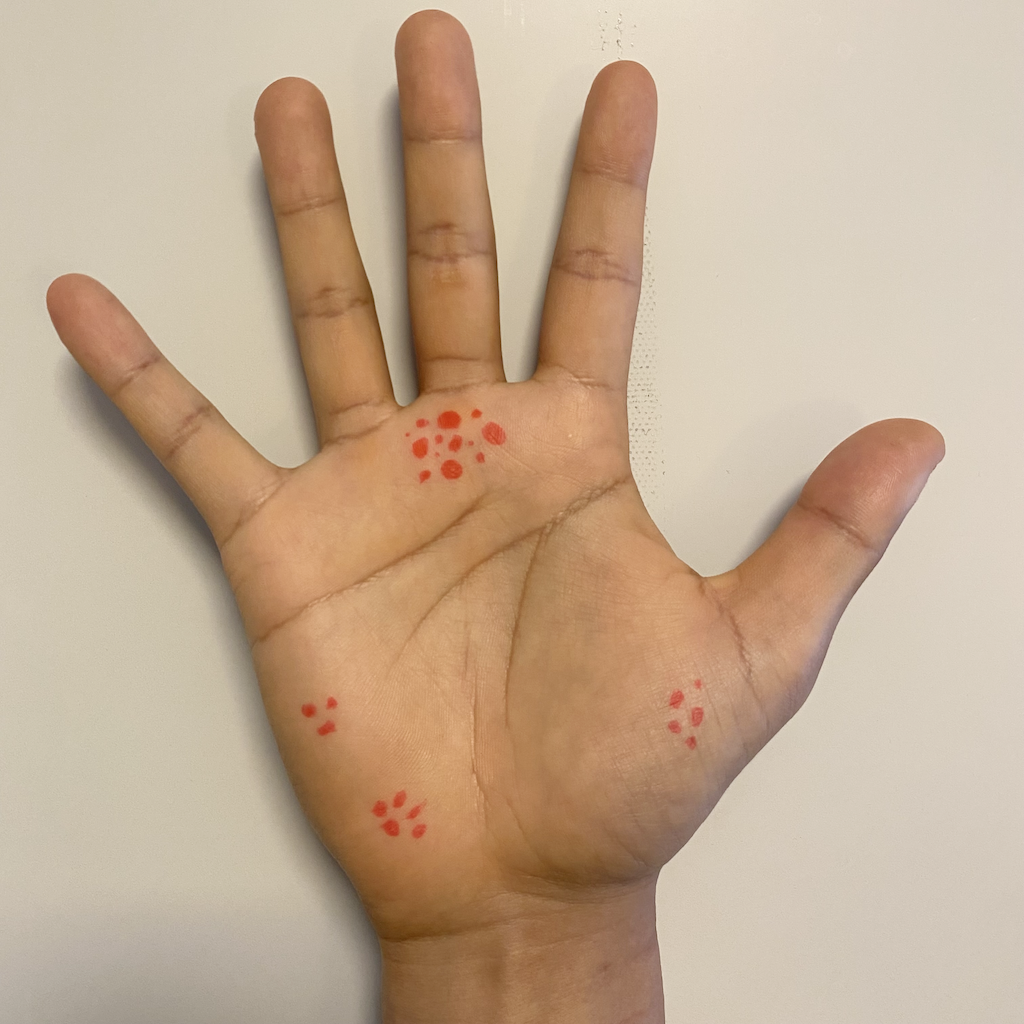
\includegraphics[width=\gridimagewidth,valign=m]{img/supplementary/background/color_block/0_color_block_0.0.png} & 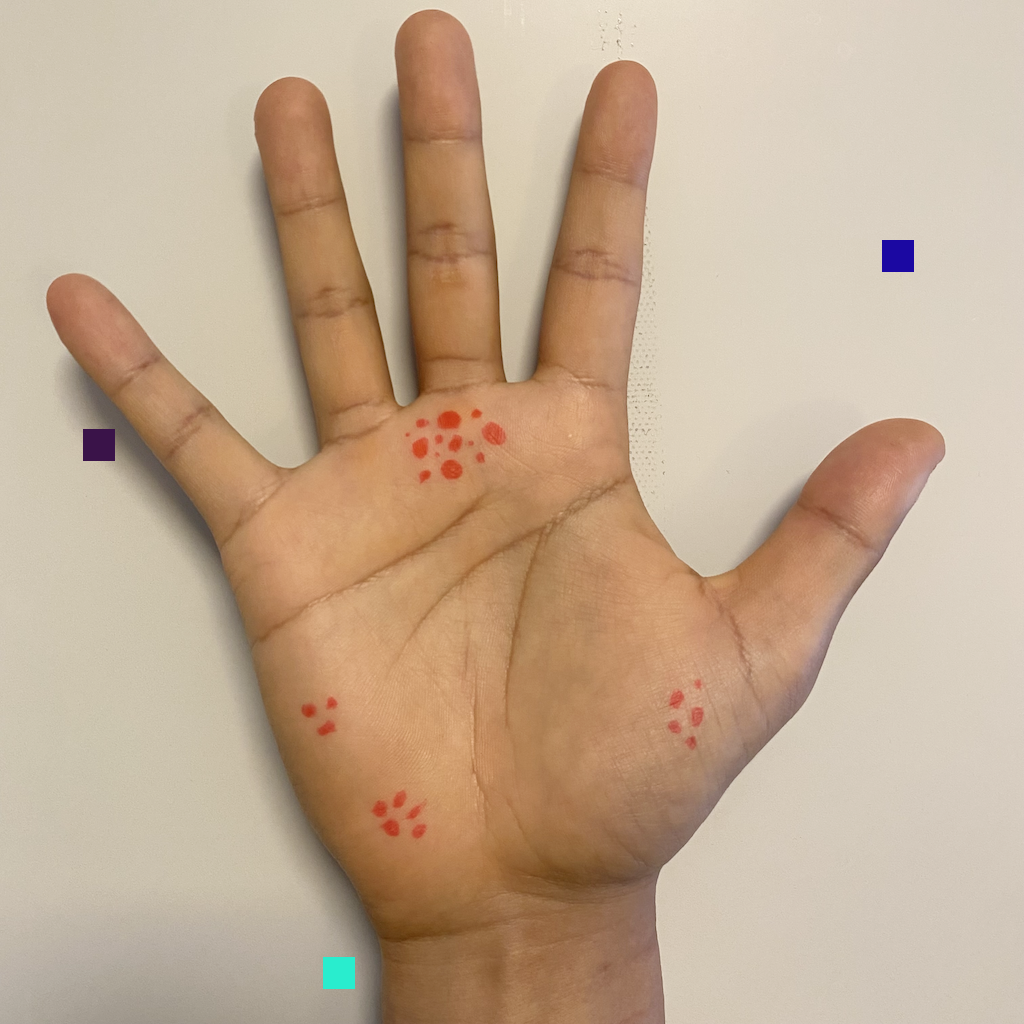
\includegraphics[width=\gridimagewidth,valign=m]{img/supplementary/background/color_block/0_color_block_0.5.png} & 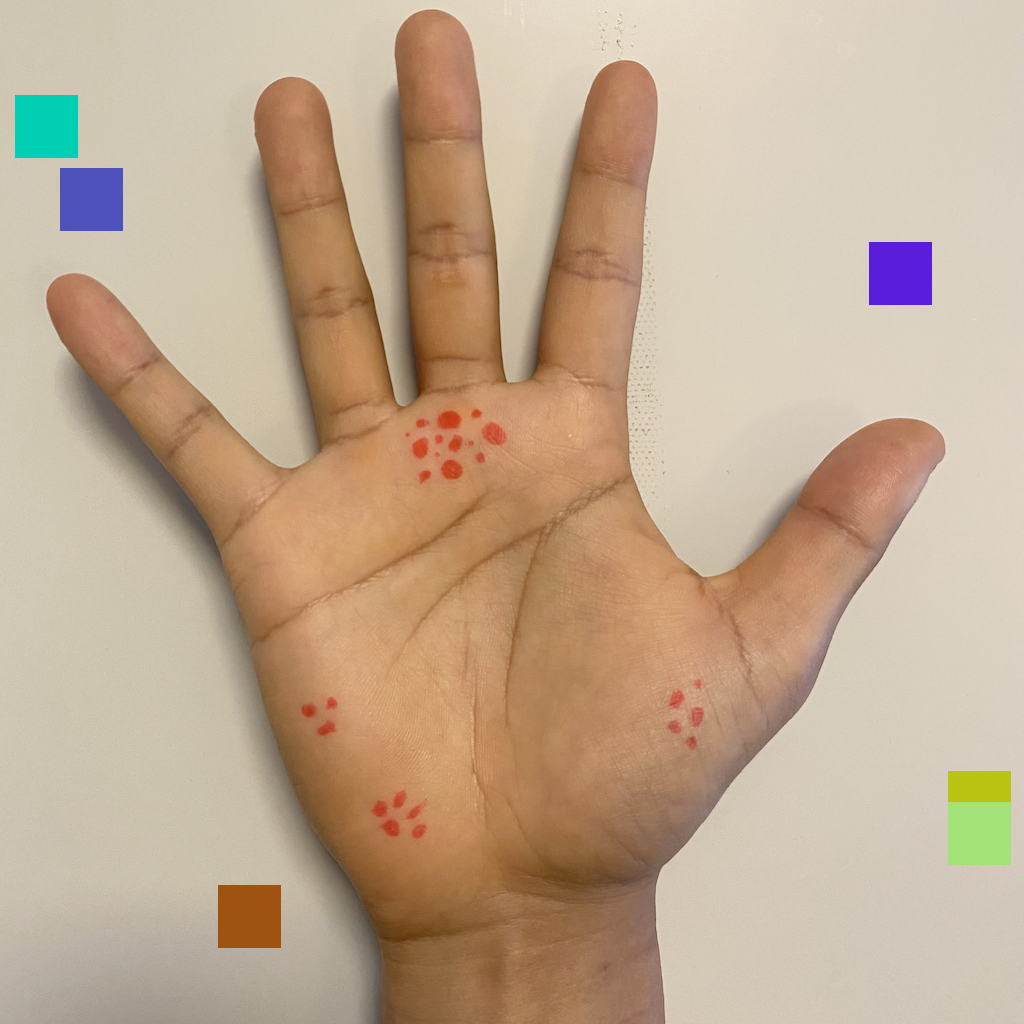
\includegraphics[width=\gridimagewidth,valign=m]{img/supplementary/background/color_block/0_color_block_1.0.png} & 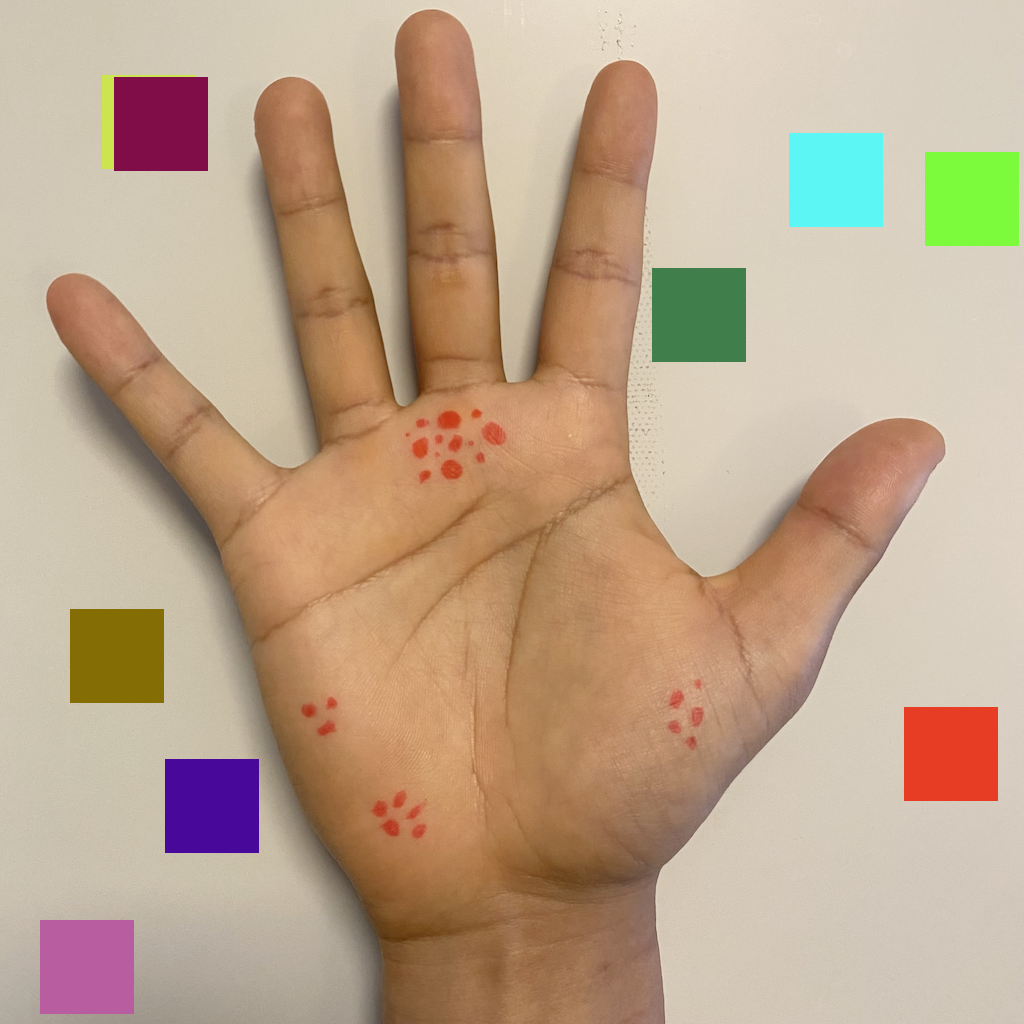
\includegraphics[width=\gridimagewidth,valign=m]{img/supplementary/background/color_block/0_color_block_1.5.png} & 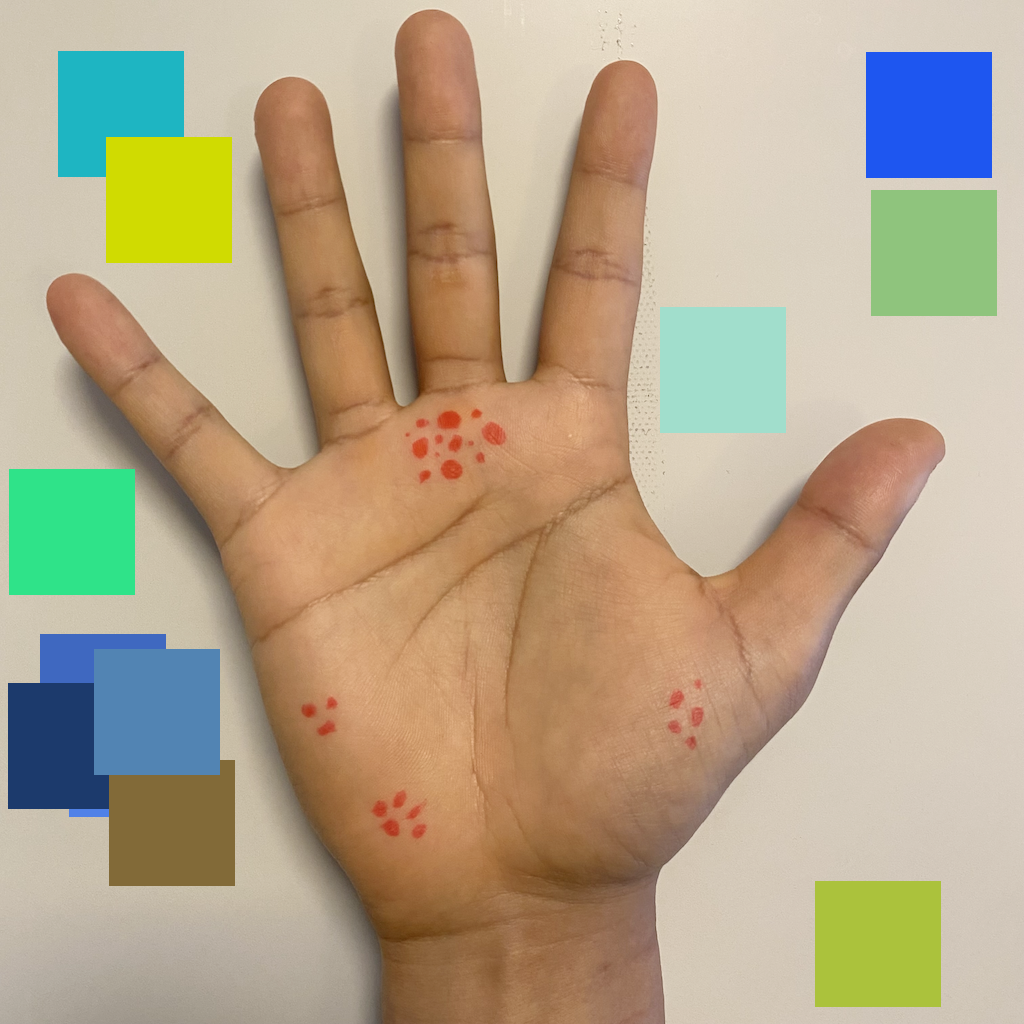
\includegraphics[width=\gridimagewidth,valign=m]{img/supplementary/background/color_block/0_color_block_2.0.png} \\ [6.15ex]
        \end{tabular}
    }
    \caption{Visualization of the degradation types belonging to the \textit{Brightness change} group for increasing levels of intensity.}
    \label{fig:background_supplementary}
\end{figure*}

\begin{figure*}
    \centering
    \setlength{\tabcolsep}{1pt}
    \Large
    \resizebox{\textwidth}{!}{%
        \begin{tabular}{C{5em}ccccc}
            & Level 1 & Level 2 & Level 3 & Level 4 & Level 5 \\
            Field of view & 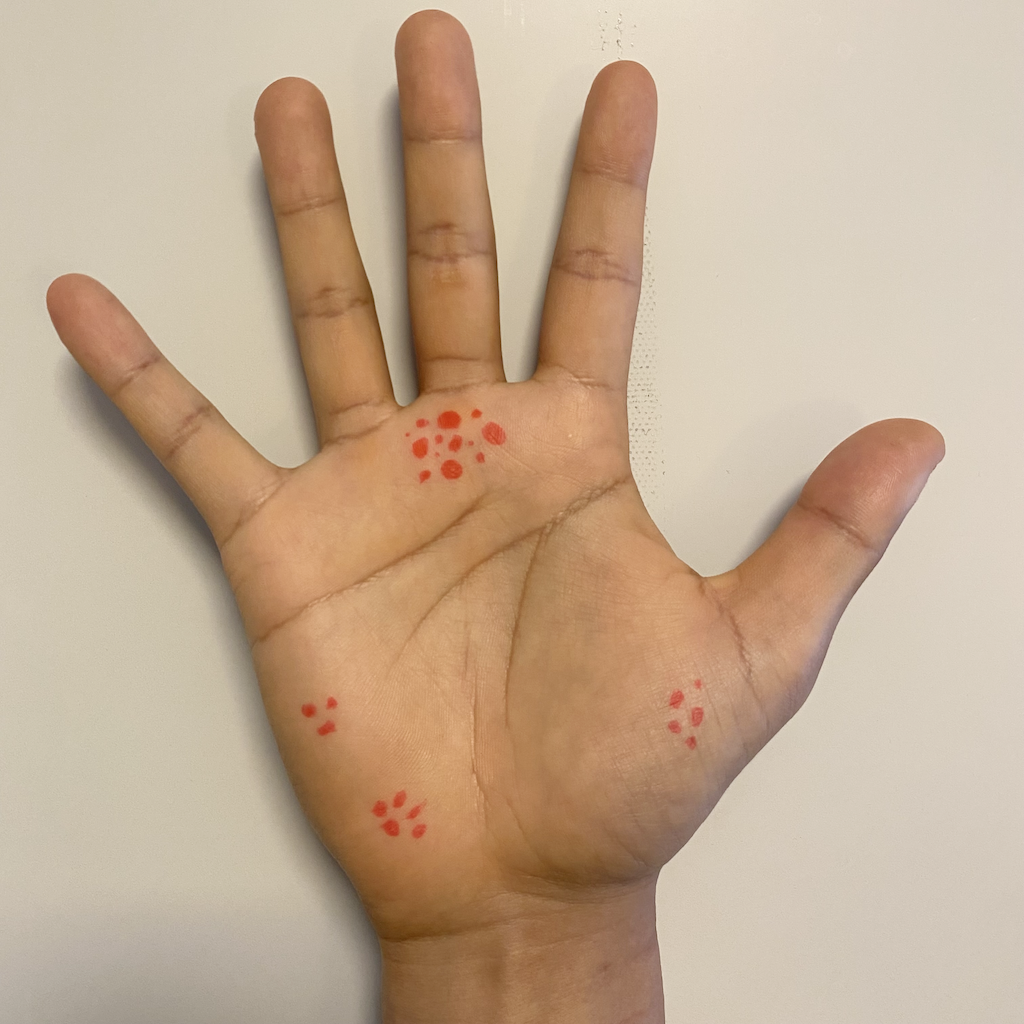
\includegraphics[width=\gridimagewidth,valign=m]{img/supplementary/field_of_view/crop_image/0_crop_image_0.png} & 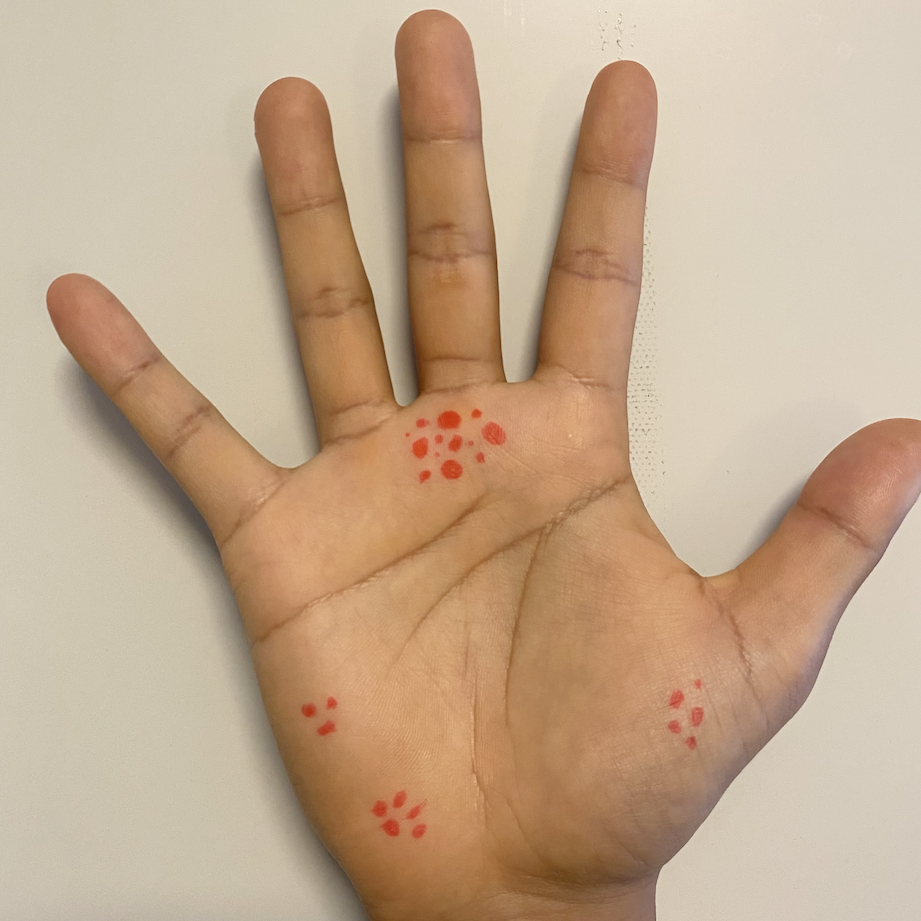
\includegraphics[width=\gridimagewidth,valign=m]{img/supplementary/field_of_view/crop_image/0_crop_image_1.png} & 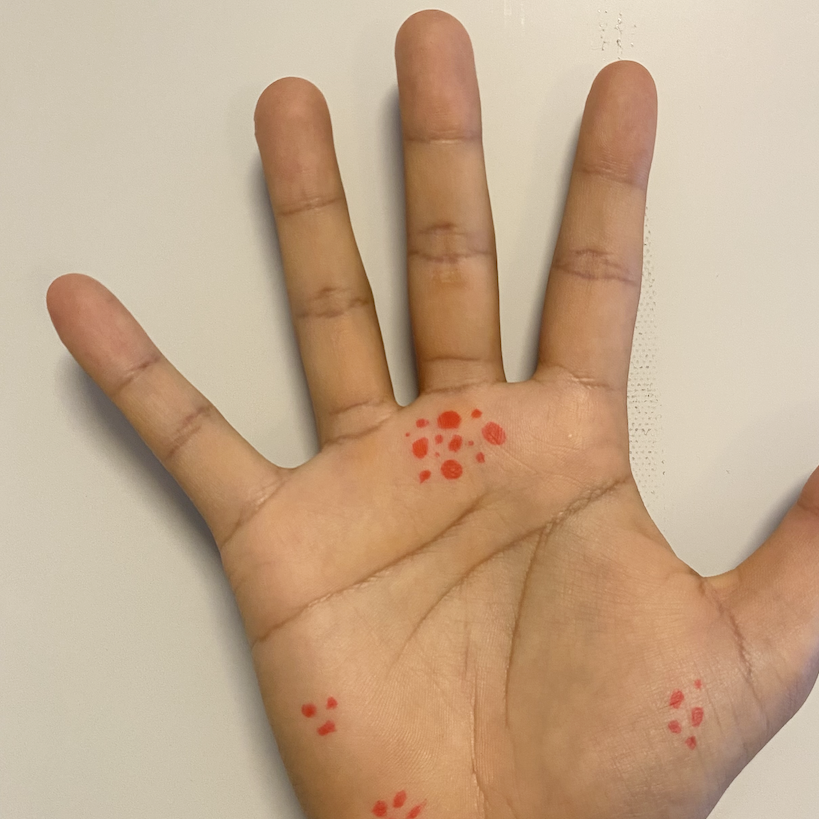
\includegraphics[width=\gridimagewidth,valign=m]{img/supplementary/field_of_view/crop_image/0_crop_image_2.png} & 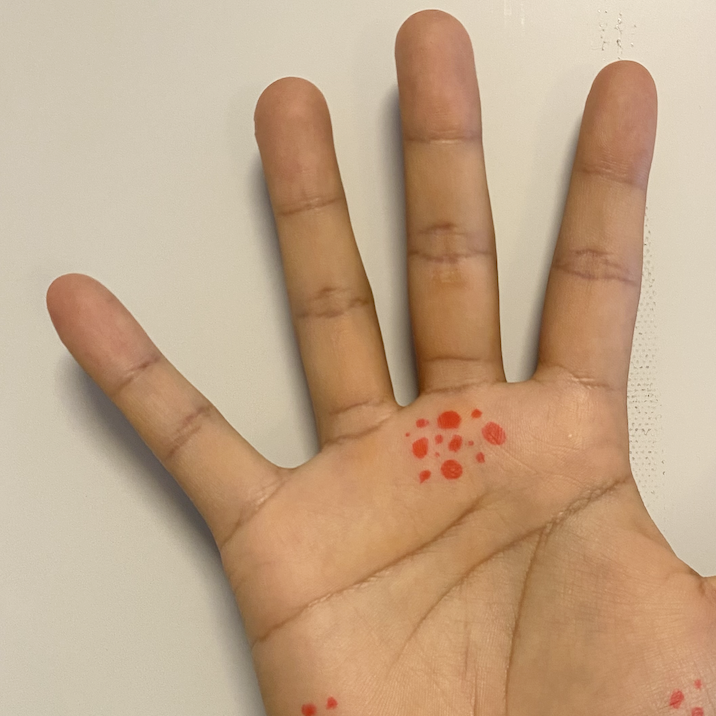
\includegraphics[width=\gridimagewidth,valign=m]{img/supplementary/field_of_view/crop_image/0_crop_image_3.png} & 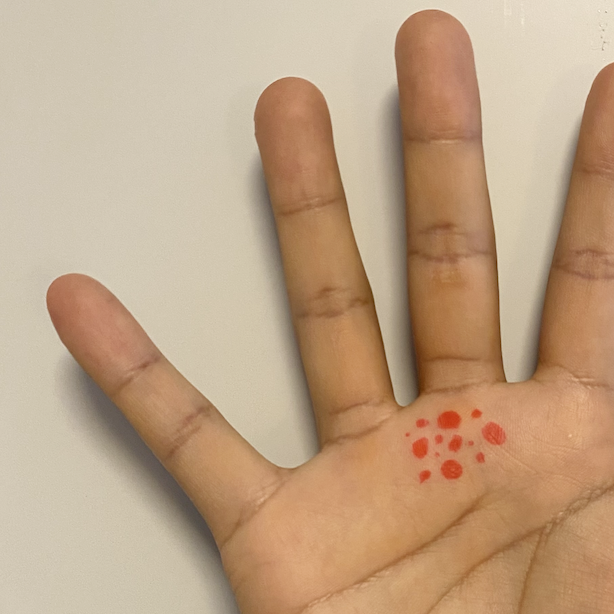
\includegraphics[width=\gridimagewidth,valign=m]{img/supplementary/field_of_view/crop_image/0_crop_image_4.png} \\ [6.15ex]
        \end{tabular}
    }
    \caption{Visualization of the degradation types belonging to the \textit{Brightness change} group for increasing levels of intensity.}
    \label{fig:field_of_view_supplementary}
\end{figure*}

\begin{figure*}
    \centering
    \setlength{\tabcolsep}{1pt}
    \Large
    \resizebox{\textwidth}{!}{%
        \begin{tabular}{C{5em}ccccc}
            & Level 1 & Level 2 & Level 3 & Level 4 & Level 5 \\
            Perspective bottom & 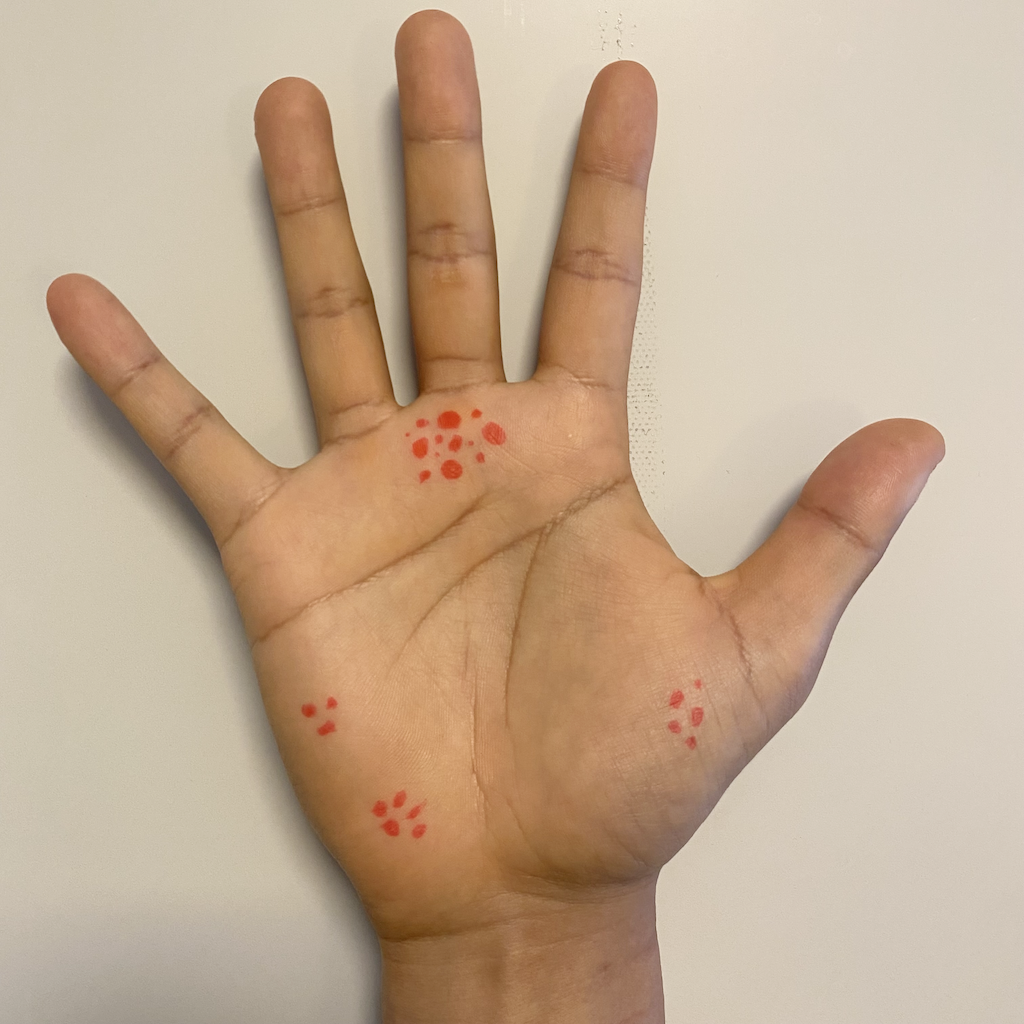
\includegraphics[width=\gridimagewidth,valign=m]{img/supplementary/orientation/perspective_bottom/0_perspective_bottom_0.0.png} & 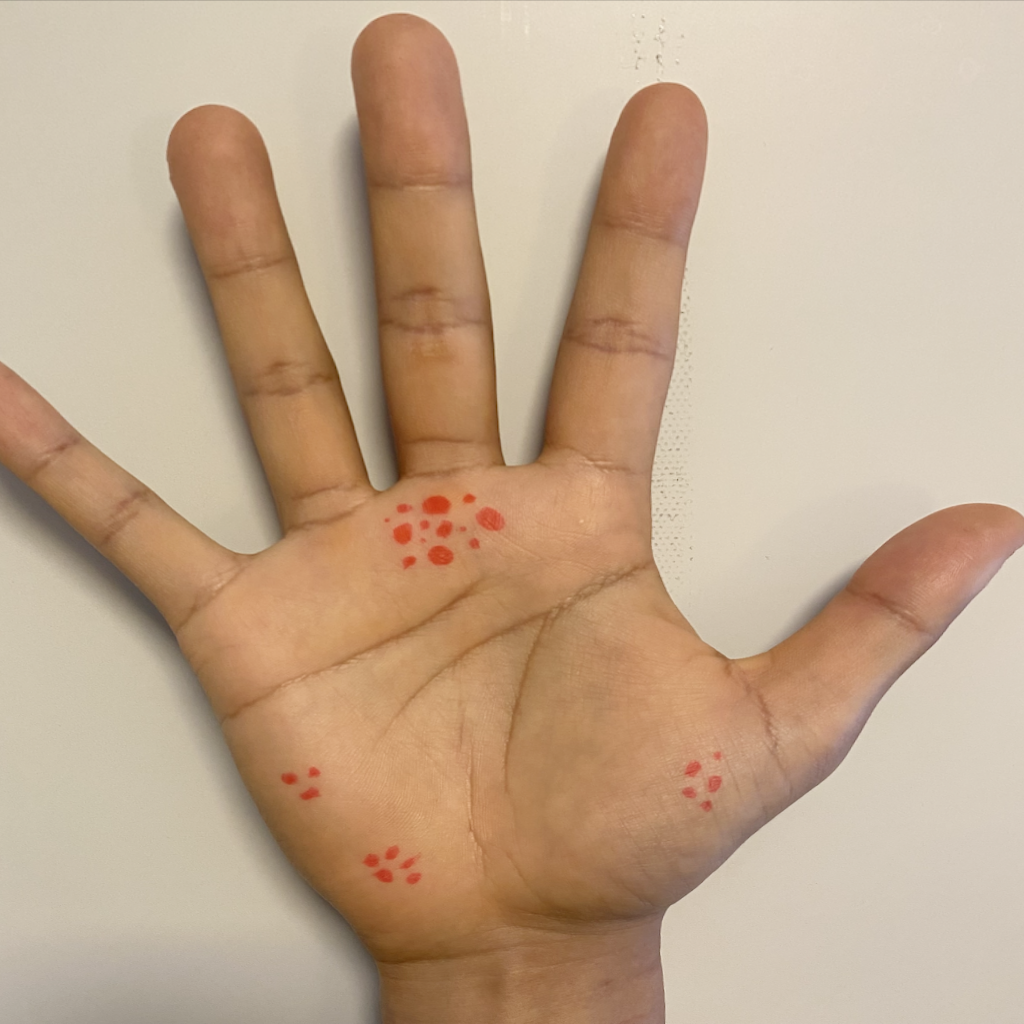
\includegraphics[width=\gridimagewidth,valign=m]{img/supplementary/orientation/perspective_bottom/0_perspective_bottom_0.2.png} & 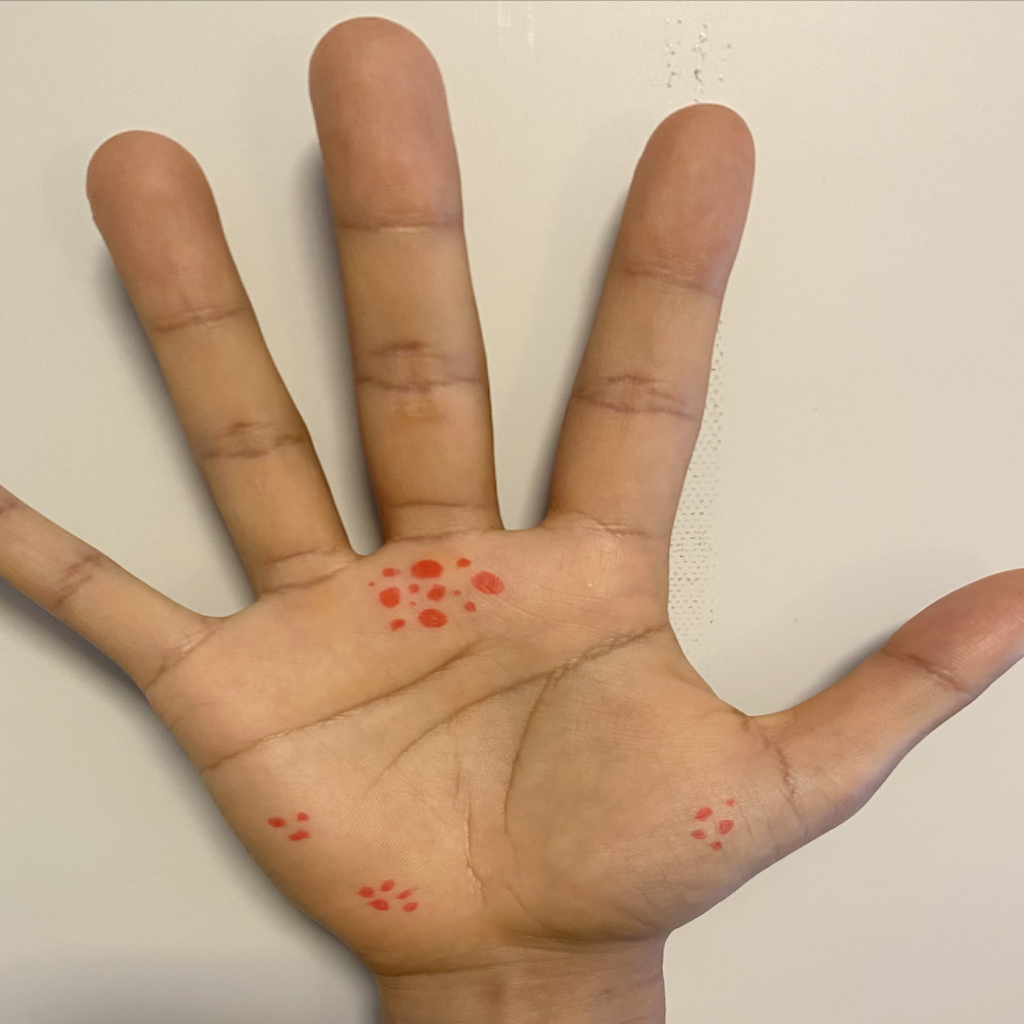
\includegraphics[width=\gridimagewidth,valign=m]{img/supplementary/orientation/perspective_bottom/0_perspective_bottom_0.4.png} & 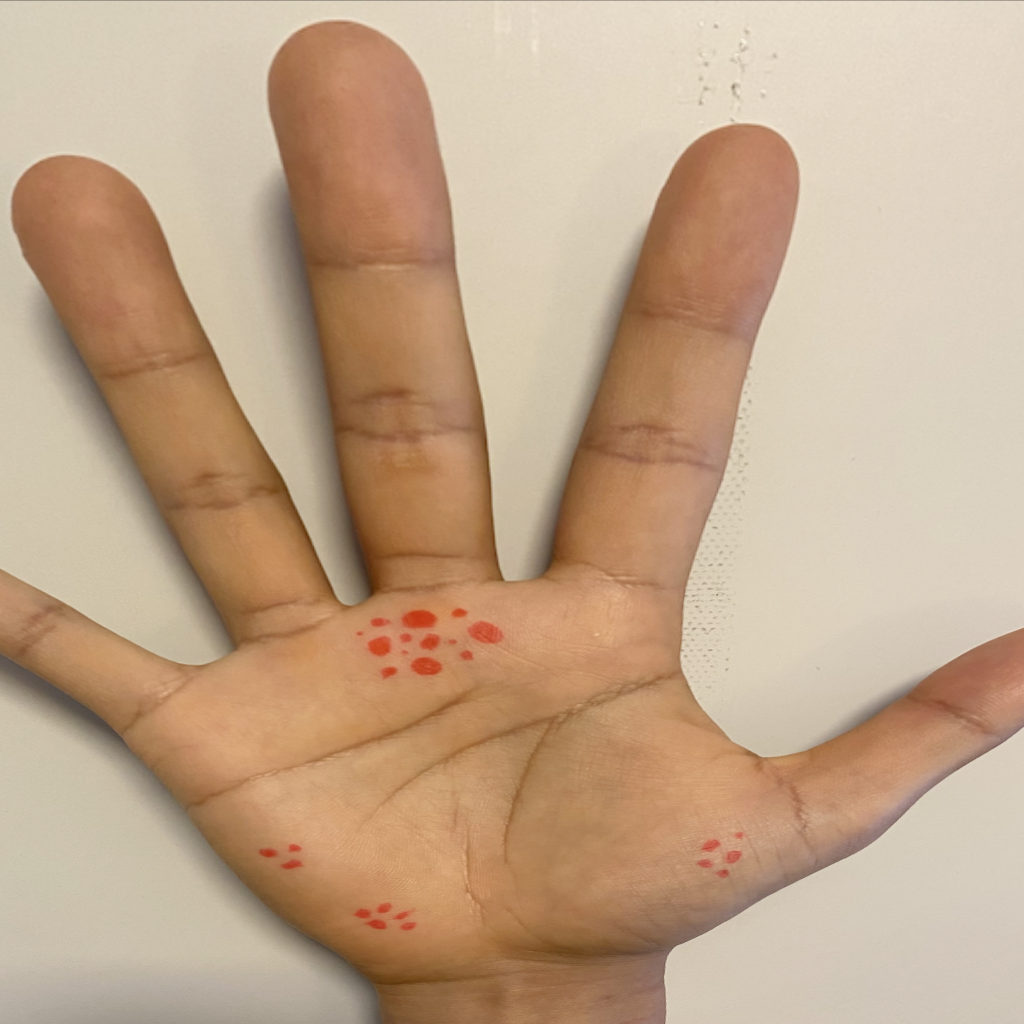
\includegraphics[width=\gridimagewidth,valign=m]{img/supplementary/orientation/perspective_bottom/0_perspective_bottom_0.6.png} & 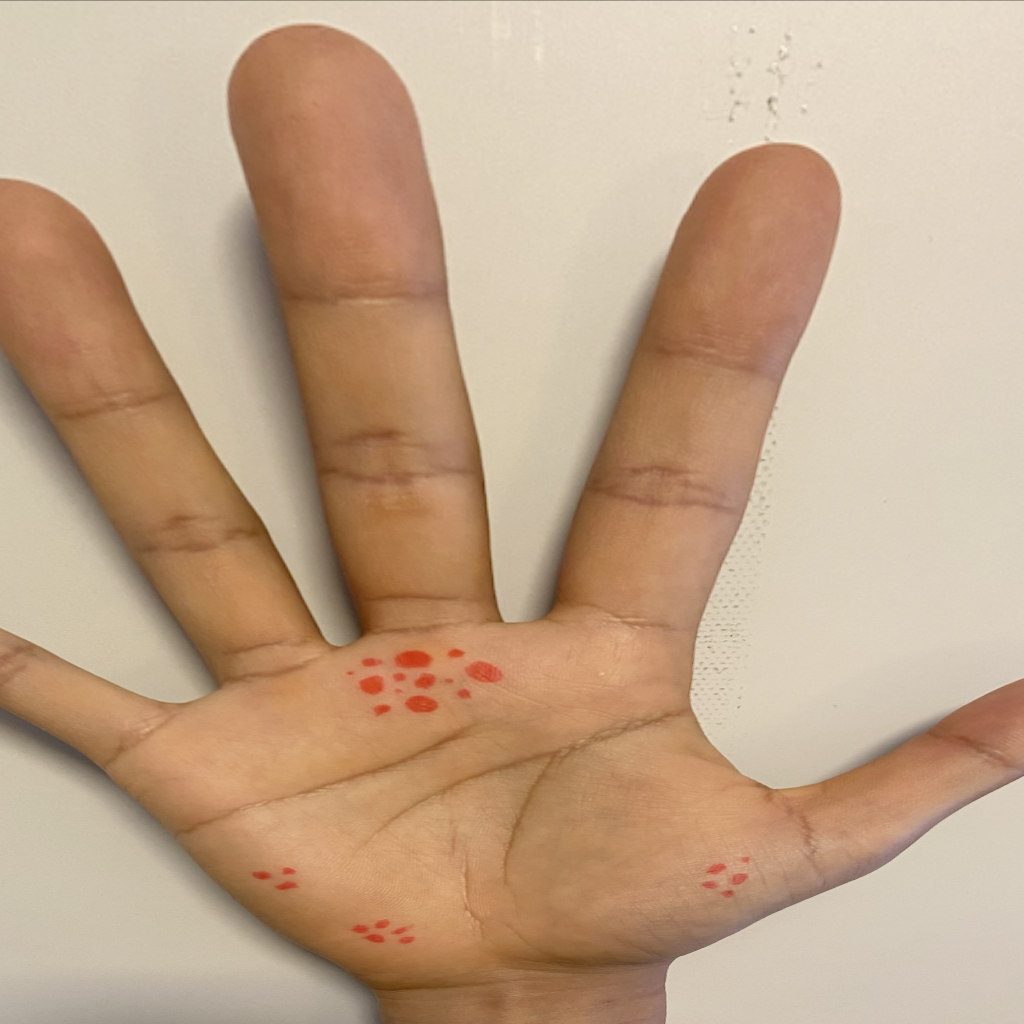
\includegraphics[width=\gridimagewidth,valign=m]{img/supplementary/orientation/perspective_bottom/0_perspective_bottom_0.8.png} \\ [6.15ex]
            Perspective top & 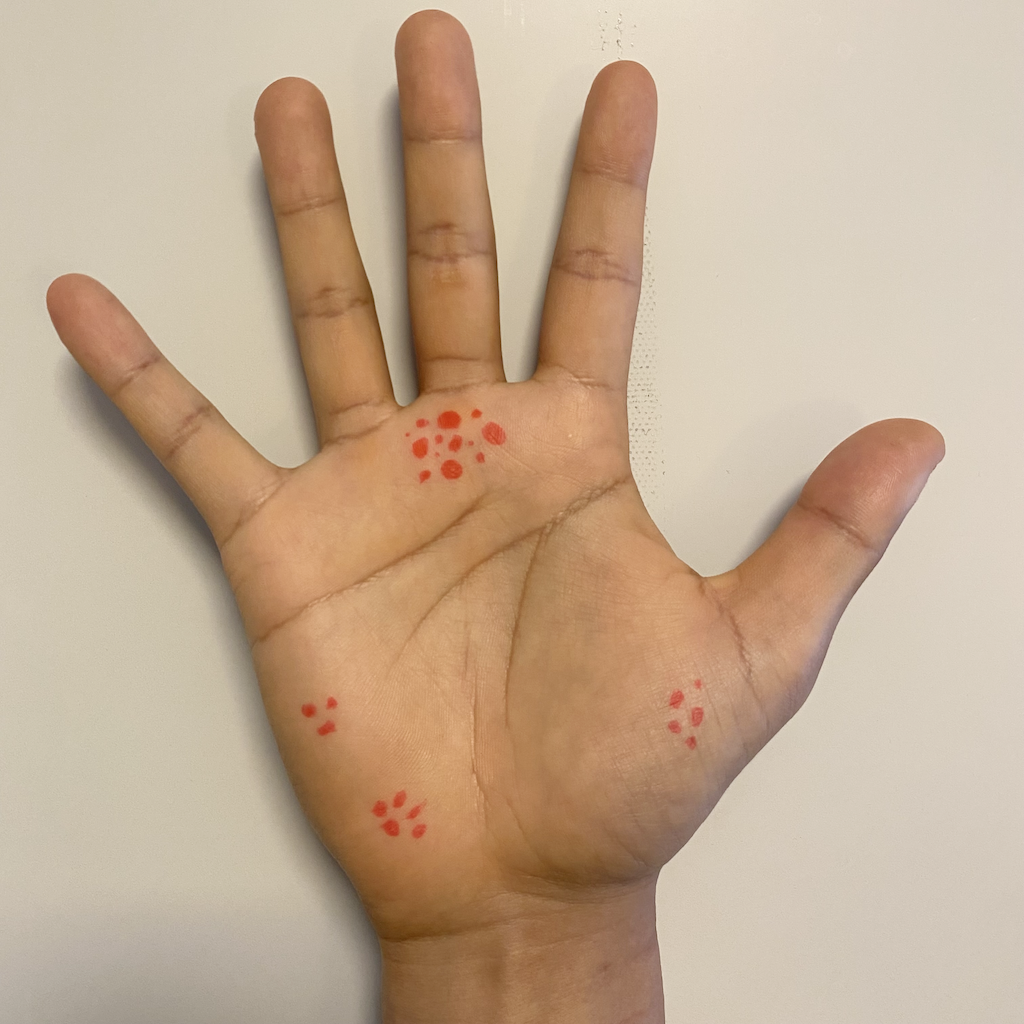
\includegraphics[width=\gridimagewidth,valign=m]{img/supplementary/orientation/perspective_top/0_perspective_top_0.0.png} & 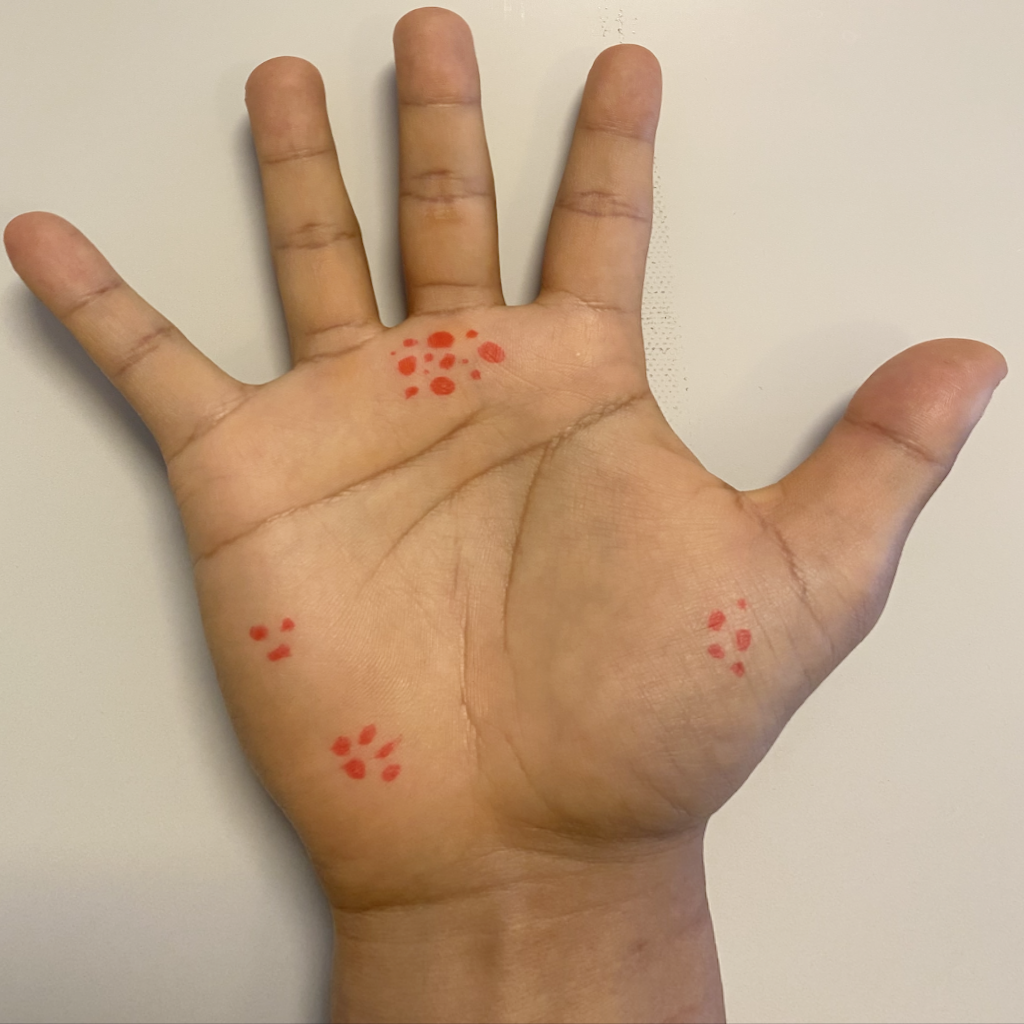
\includegraphics[width=\gridimagewidth,valign=m]{img/supplementary/orientation/perspective_top/0_perspective_top_0.2.png} & 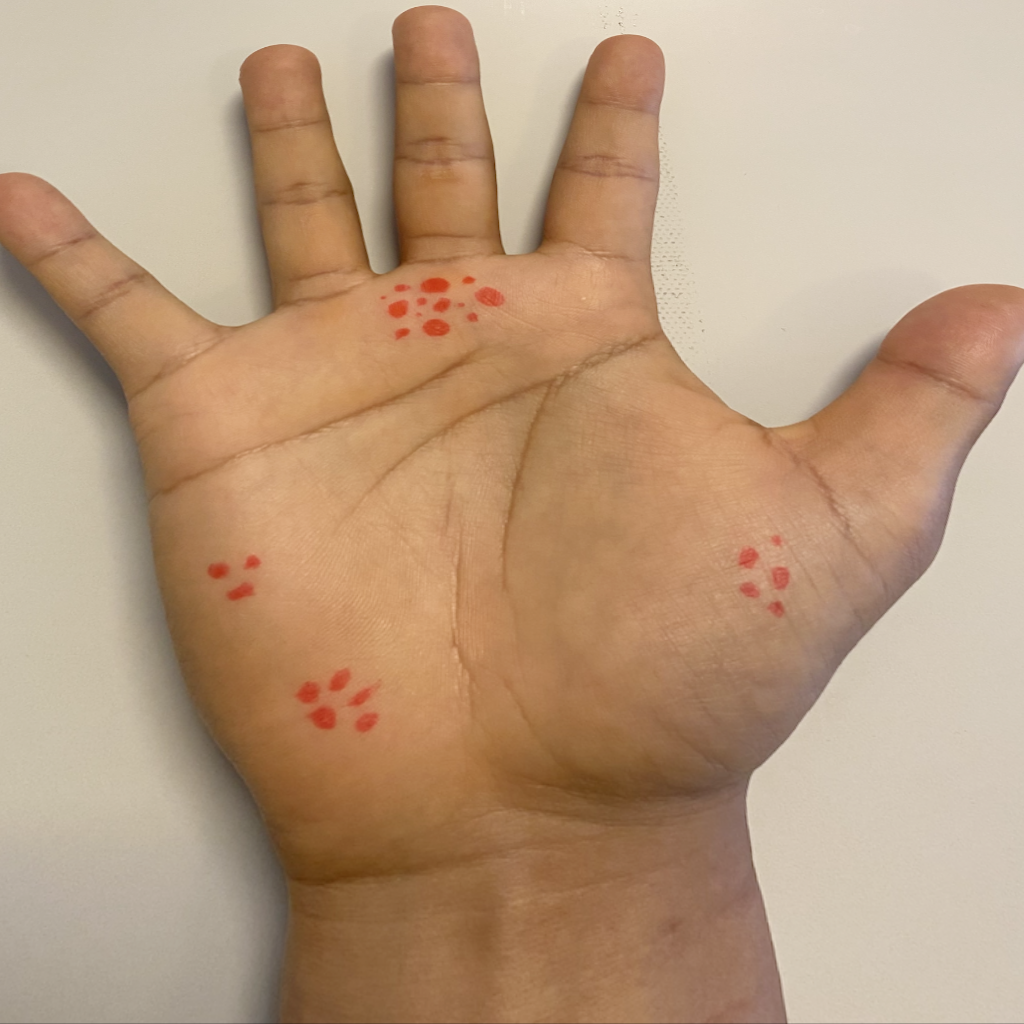
\includegraphics[width=\gridimagewidth,valign=m]{img/supplementary/orientation/perspective_top/0_perspective_top_0.4.png} & 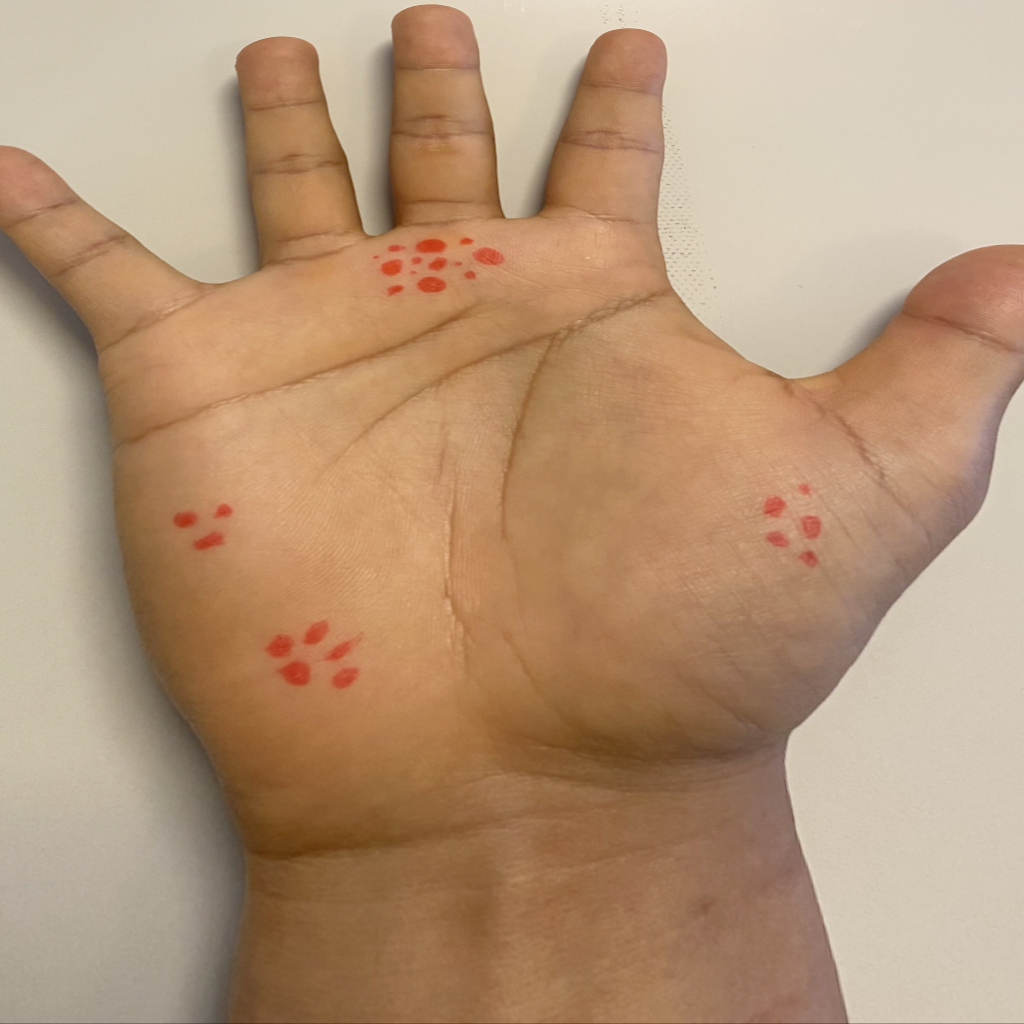
\includegraphics[width=\gridimagewidth,valign=m]{img/supplementary/orientation/perspective_top/0_perspective_top_0.6.png} & 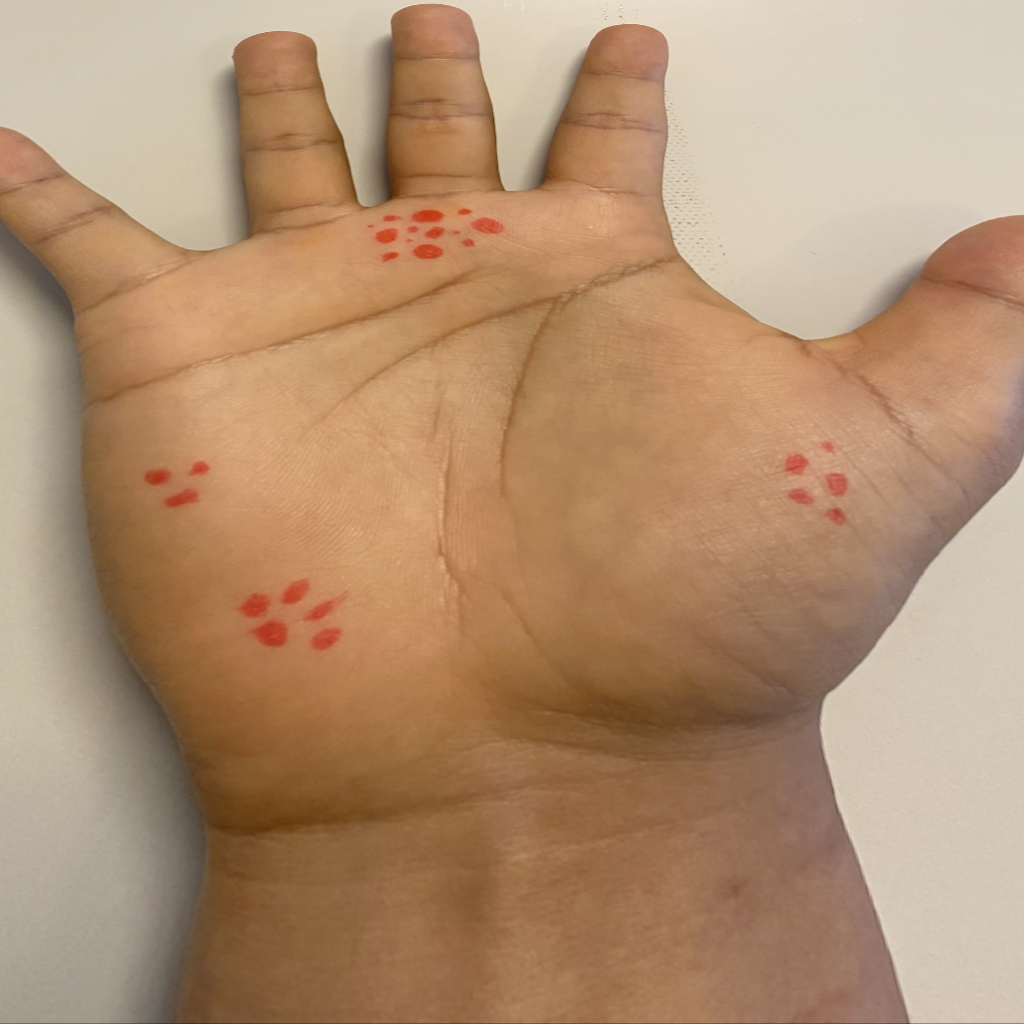
\includegraphics[width=\gridimagewidth,valign=m]{img/supplementary/orientation/perspective_top/0_perspective_top_0.8.png} \\ [6.15ex]
            Perspective left & 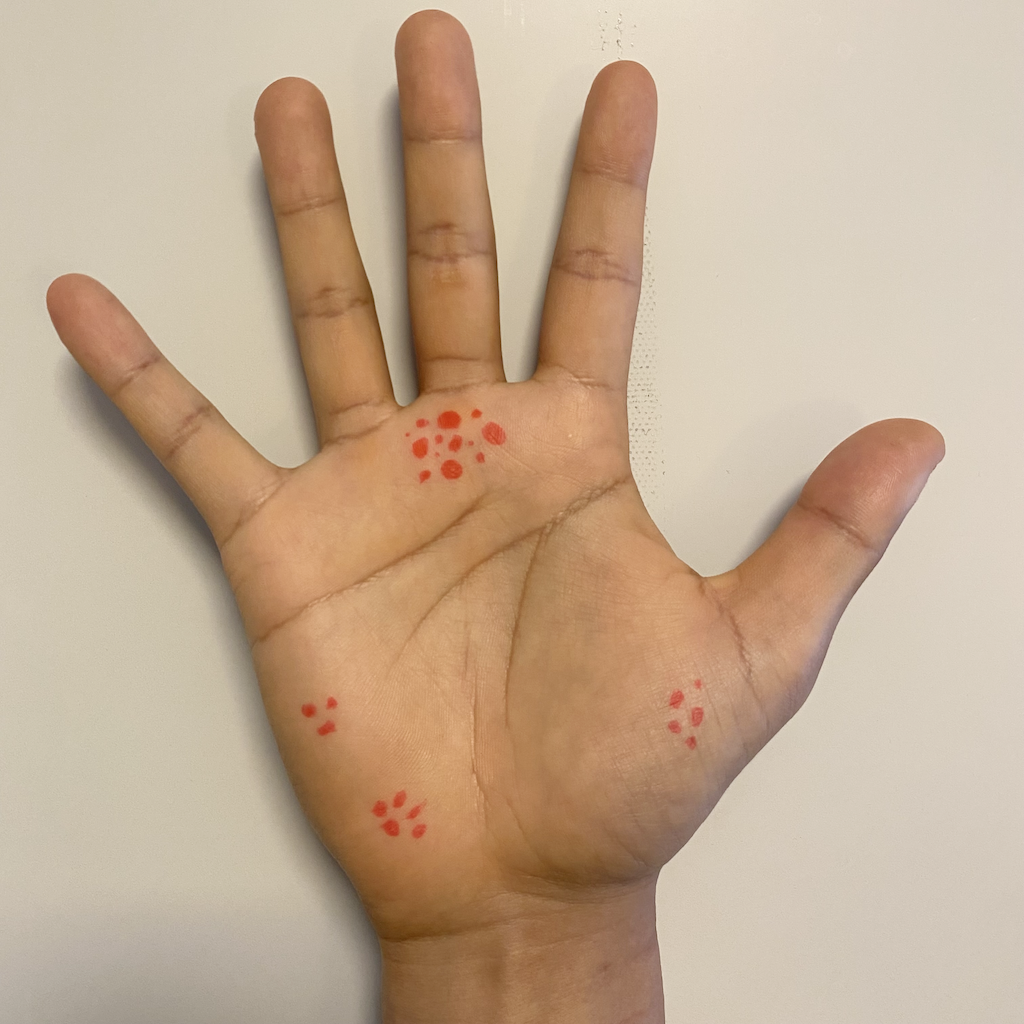
\includegraphics[width=\gridimagewidth,valign=m]{img/supplementary/orientation/perspective_left/0_perspective_left_0.0.png} & 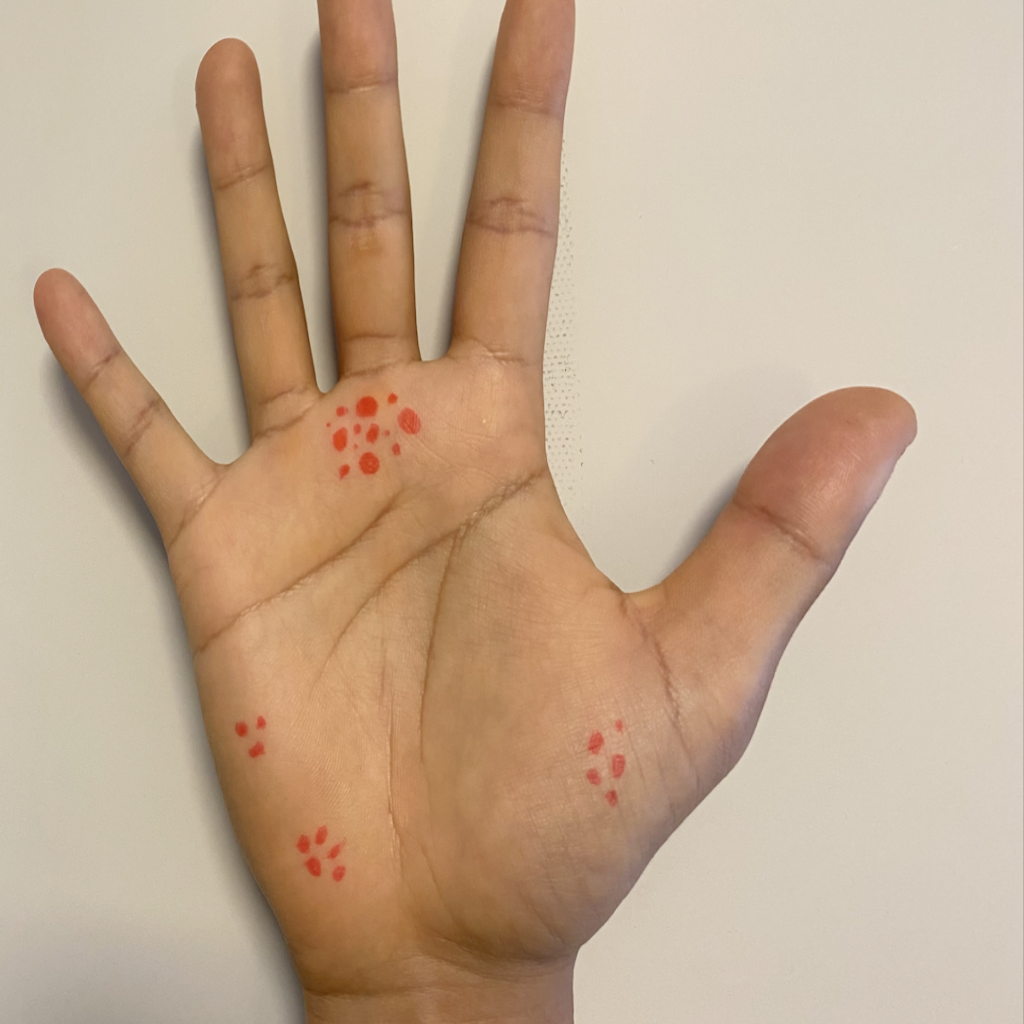
\includegraphics[width=\gridimagewidth,valign=m]{img/supplementary/orientation/perspective_left/0_perspective_left_0.2.png} & 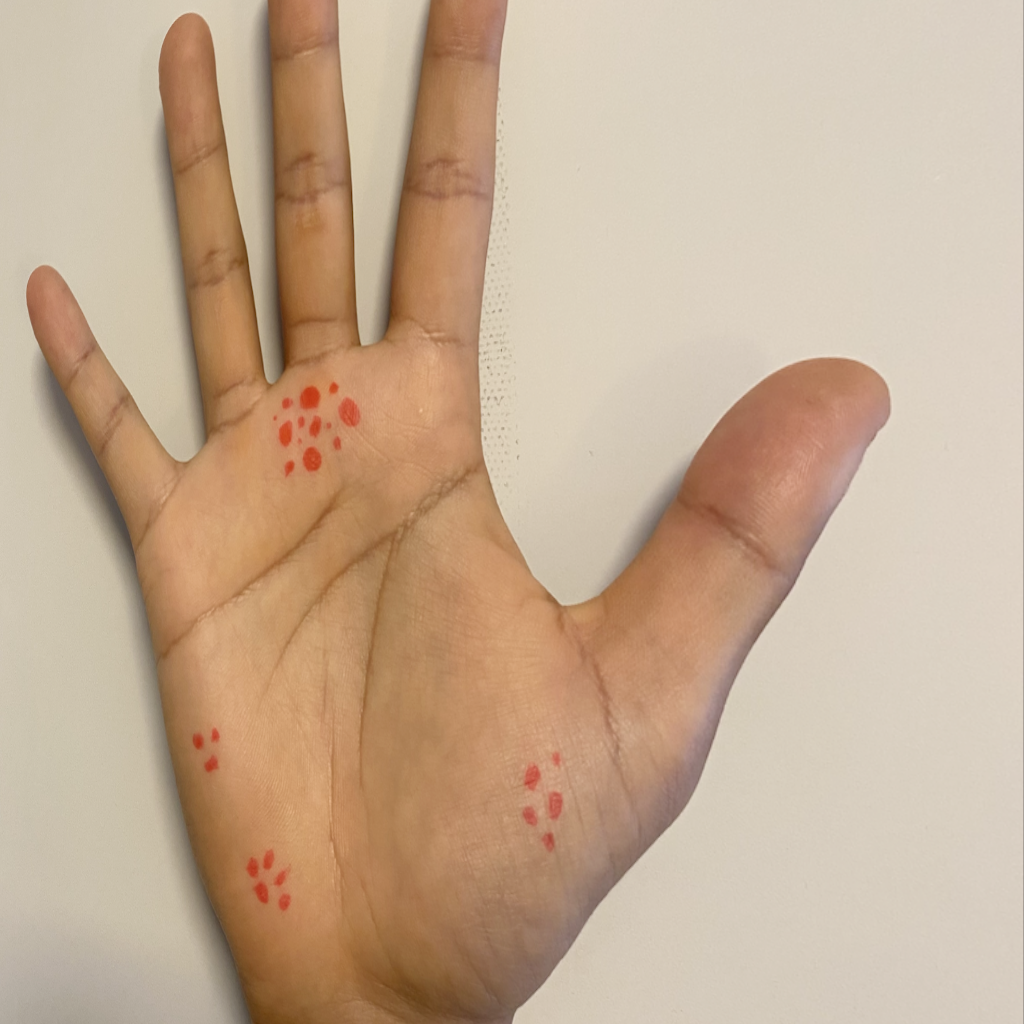
\includegraphics[width=\gridimagewidth,valign=m]{img/supplementary/orientation/perspective_left/0_perspective_left_0.4.png} & 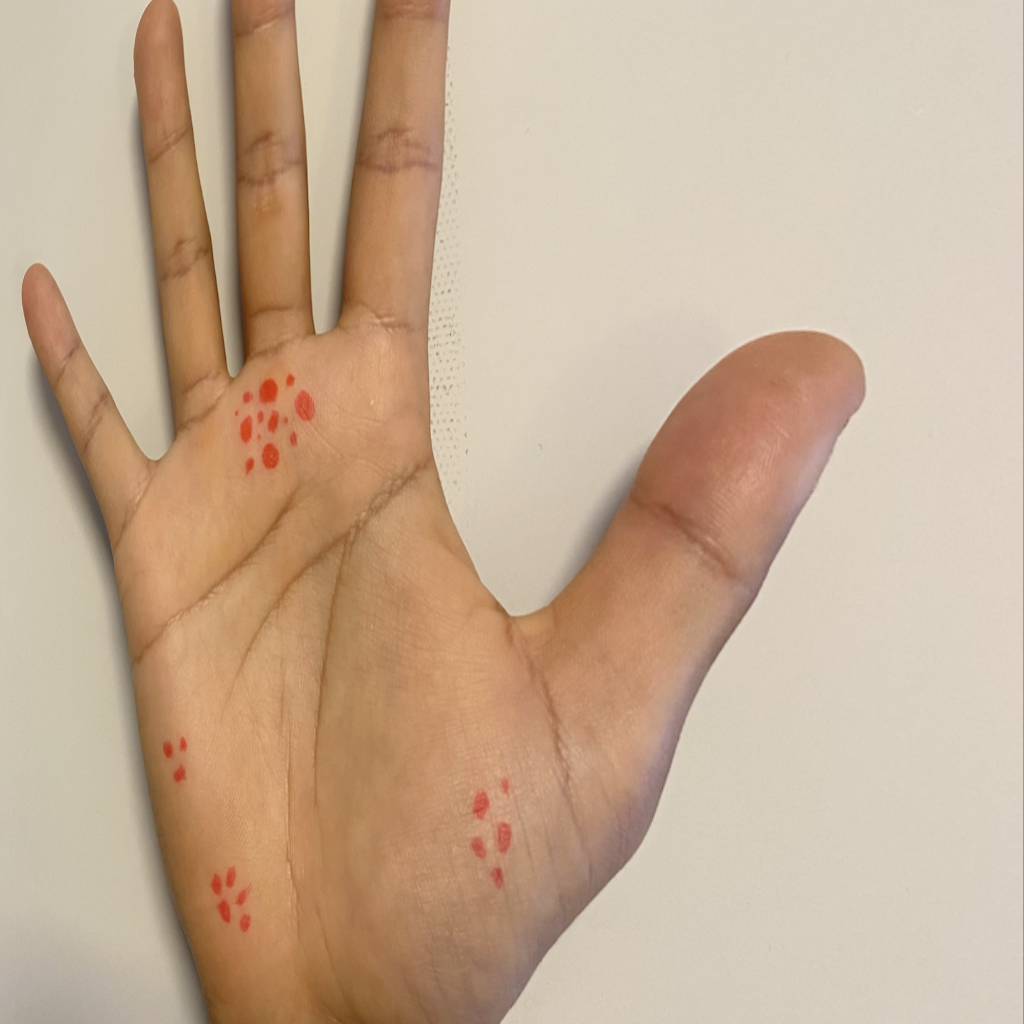
\includegraphics[width=\gridimagewidth,valign=m]{img/supplementary/orientation/perspective_left/0_perspective_left_0.6.png} & 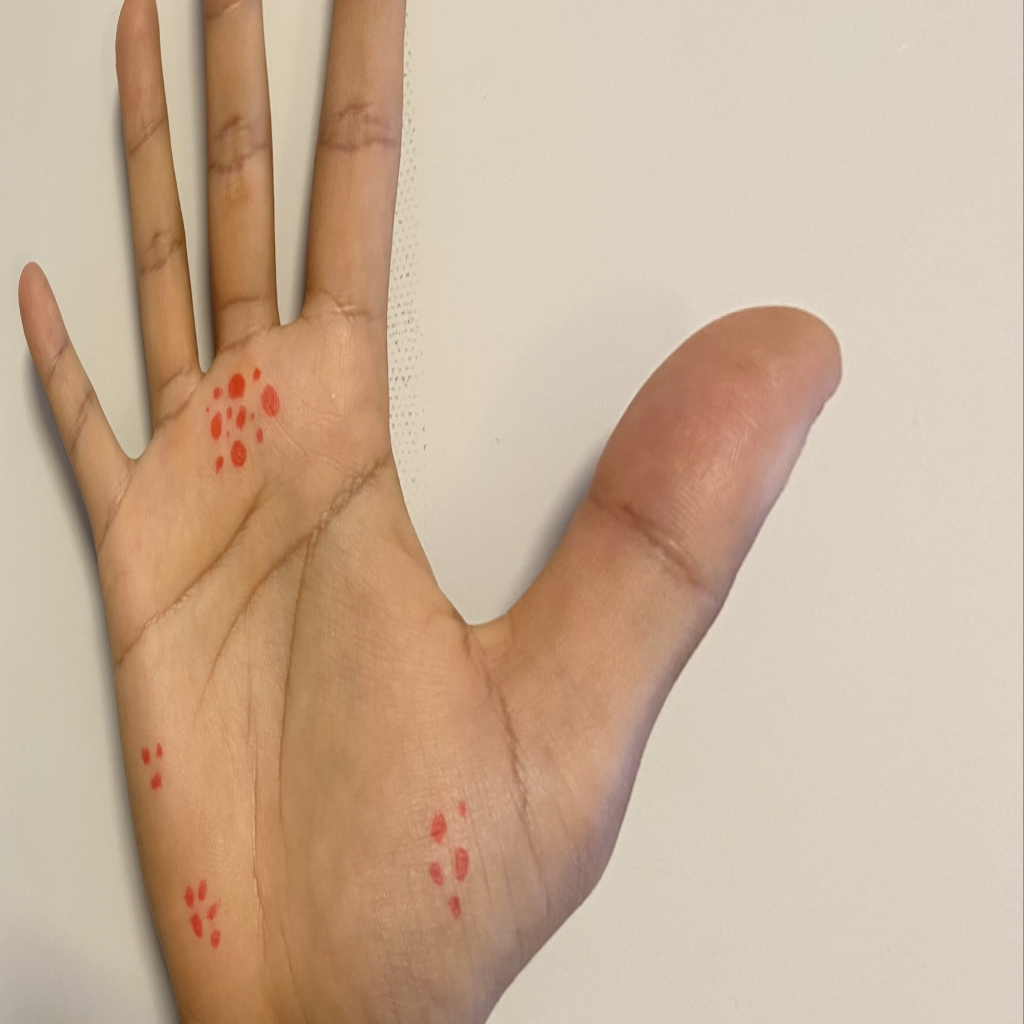
\includegraphics[width=\gridimagewidth,valign=m]{img/supplementary/orientation/perspective_left/0_perspective_left_0.8.png} \\ [6.15ex]
            Perspective right & 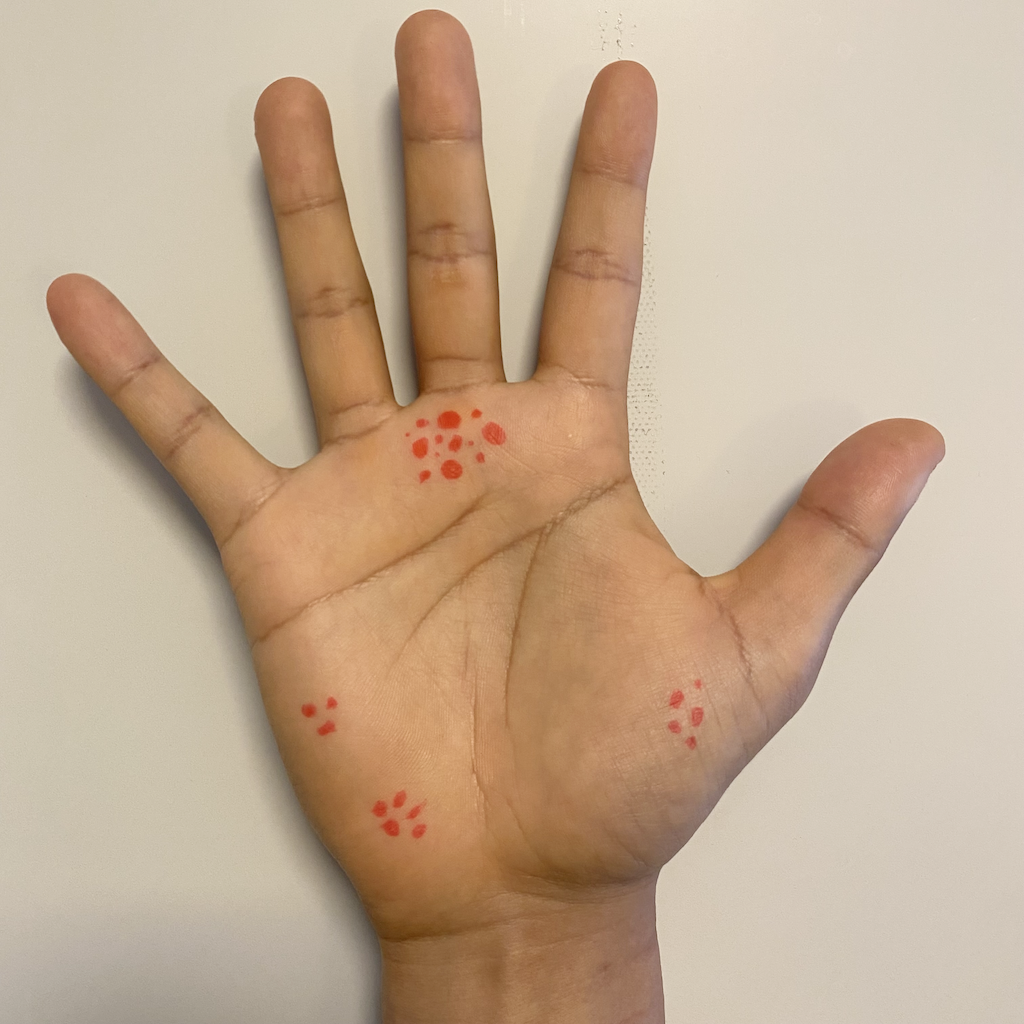
\includegraphics[width=\gridimagewidth,valign=m]{img/supplementary/orientation/perspective_right/0_perspective_right_0.0.png} & 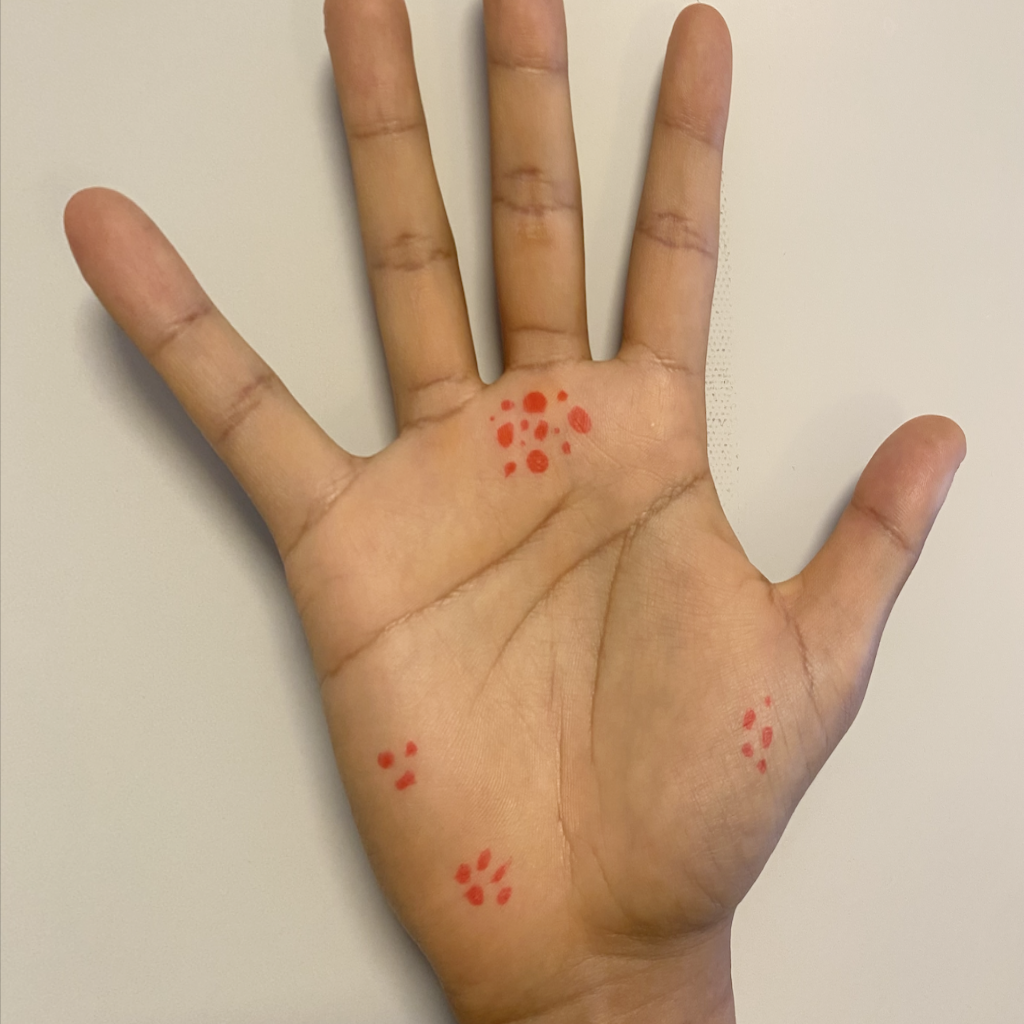
\includegraphics[width=\gridimagewidth,valign=m]{img/supplementary/orientation/perspective_right/0_perspective_right_0.2.png} & 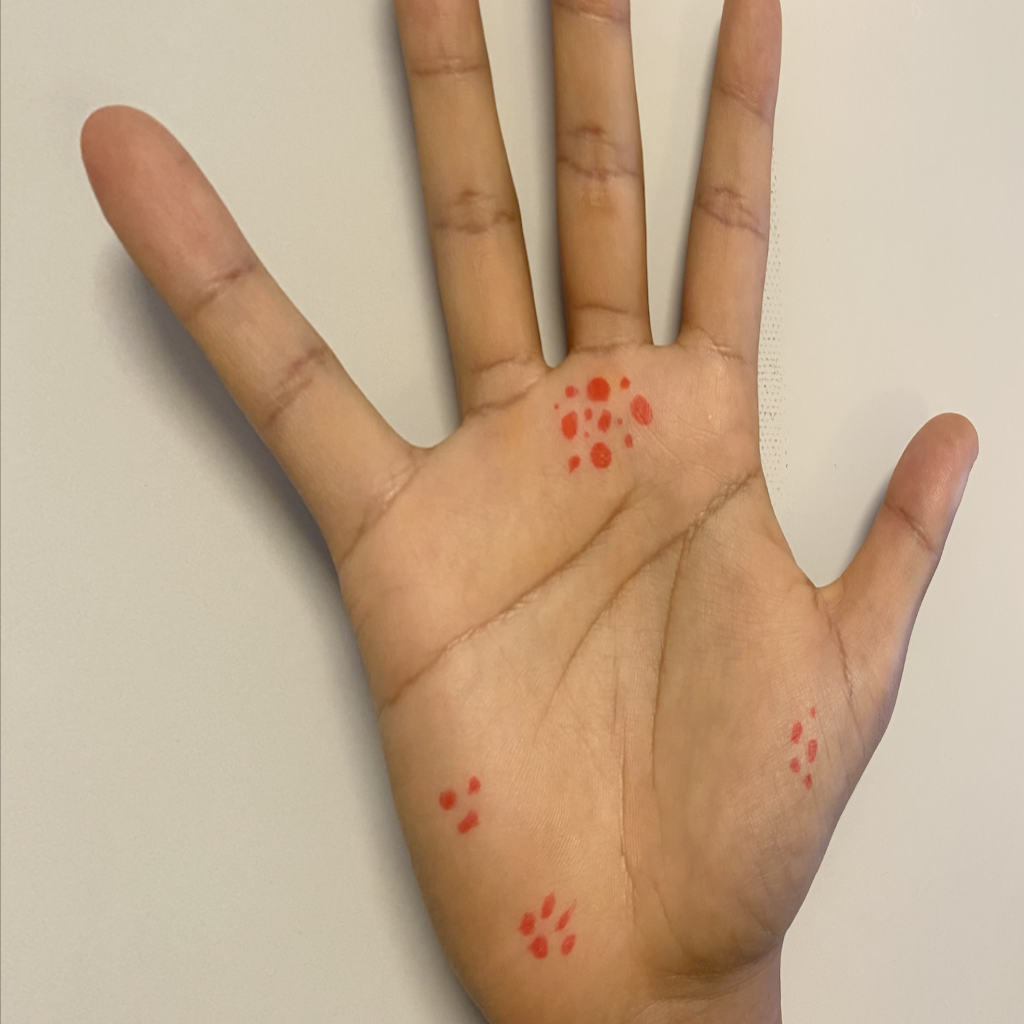
\includegraphics[width=\gridimagewidth,valign=m]{img/supplementary/orientation/perspective_right/0_perspective_right_0.4.png} & 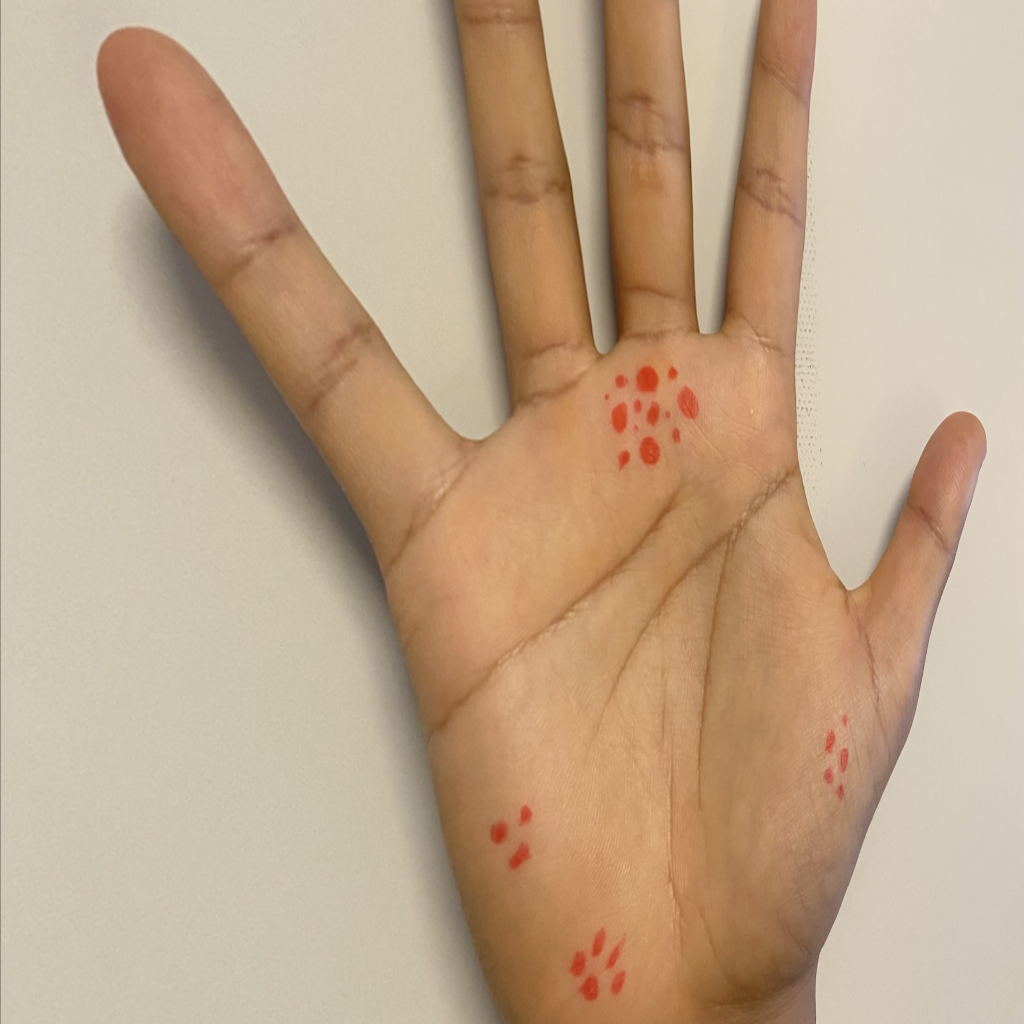
\includegraphics[width=\gridimagewidth,valign=m]{img/supplementary/orientation/perspective_right/0_perspective_right_0.6.png} & 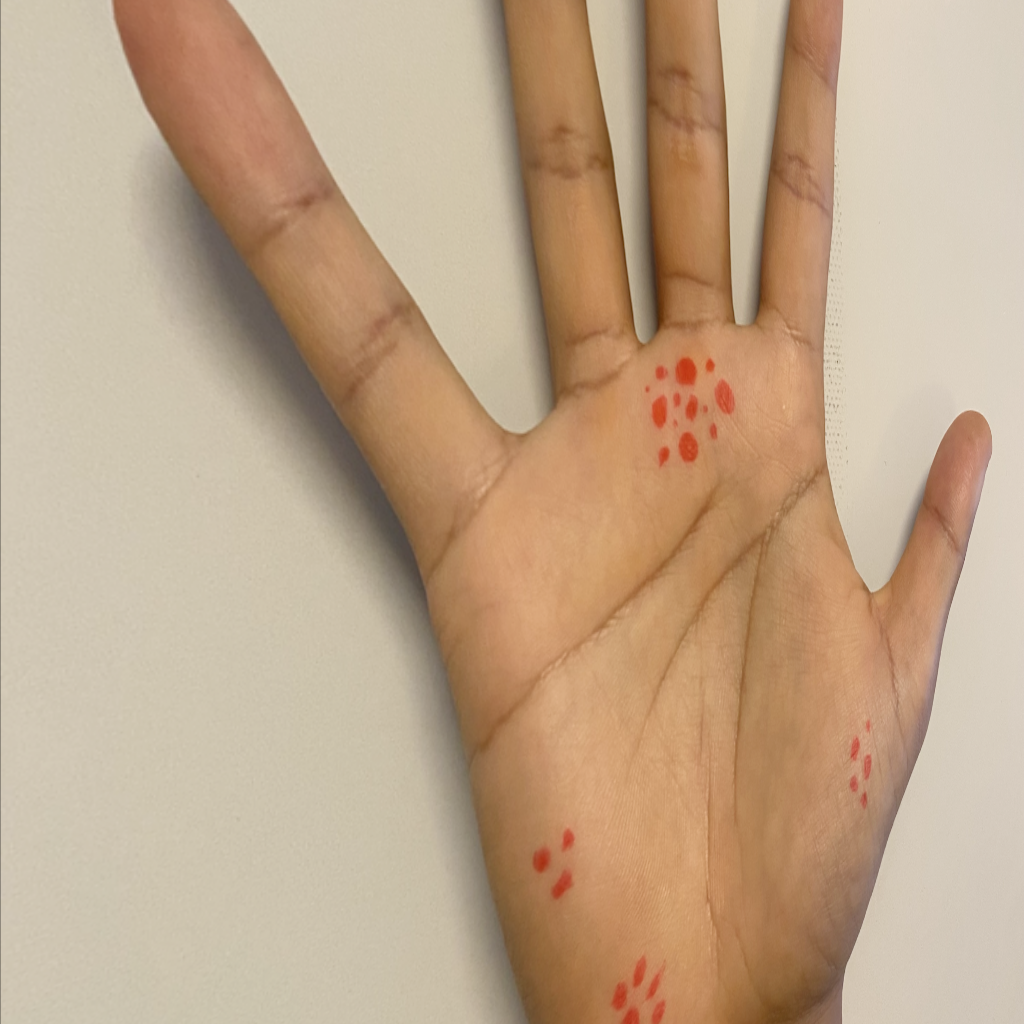
\includegraphics[width=\gridimagewidth,valign=m]{img/supplementary/orientation/perspective_right/0_perspective_right_0.8.png} \\ [6.15ex]
        \end{tabular}
    }
    \caption{Visualization of the degradation types belonging to the \textit{Brightness change} group for increasing levels of intensity.}
    \label{fig:orientation_supplementary}
\end{figure*}

\begin{figure*}
    \centering
    \setlength{\tabcolsep}{1pt}
    \Large
    \resizebox{\textwidth}{!}{%
        \begin{tabular}{C{5em}ccccc}
            & Level 1 & Level 2 & Level 3 & Level 4 & Level 5 \\
            Gaussian blur & 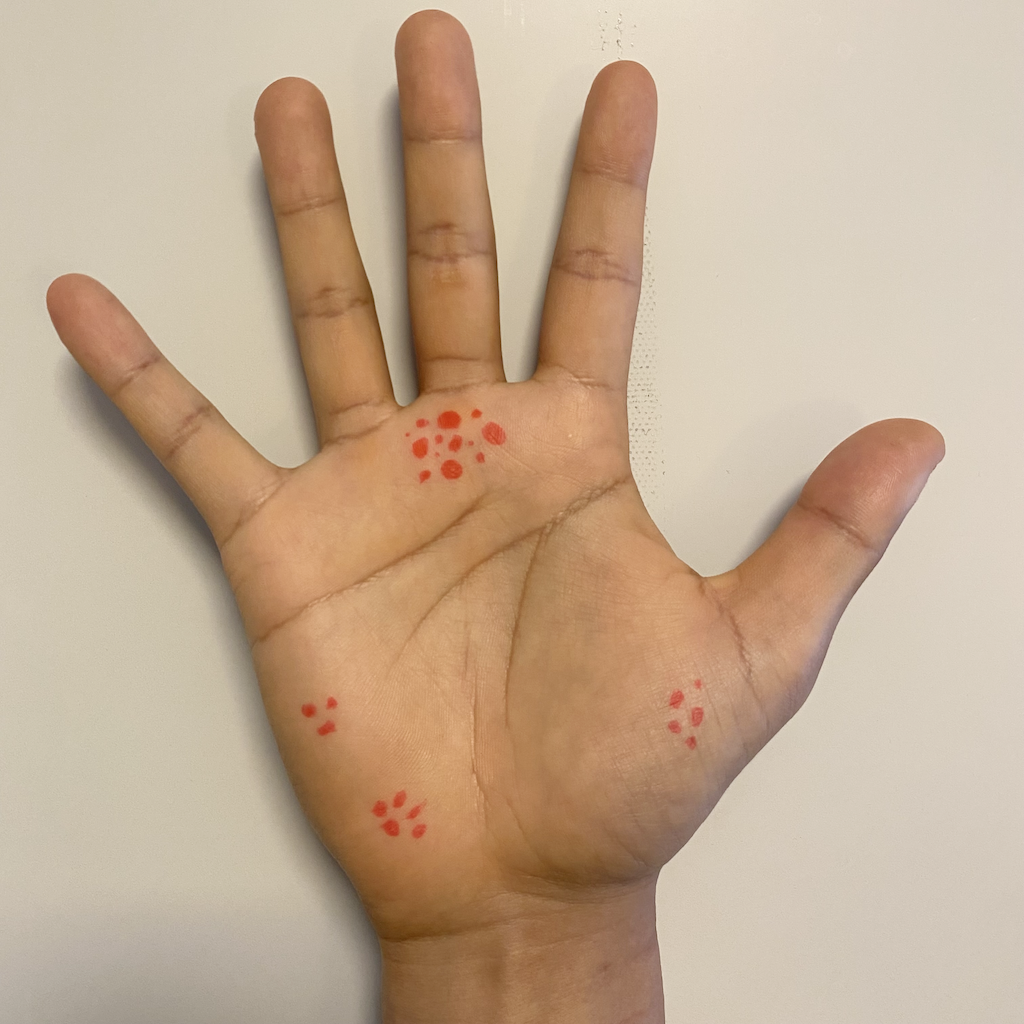
\includegraphics[width=\gridimagewidth,valign=m]{img/supplementary/focus/gaussian_blur/0_gaussian_blur_0.png} & 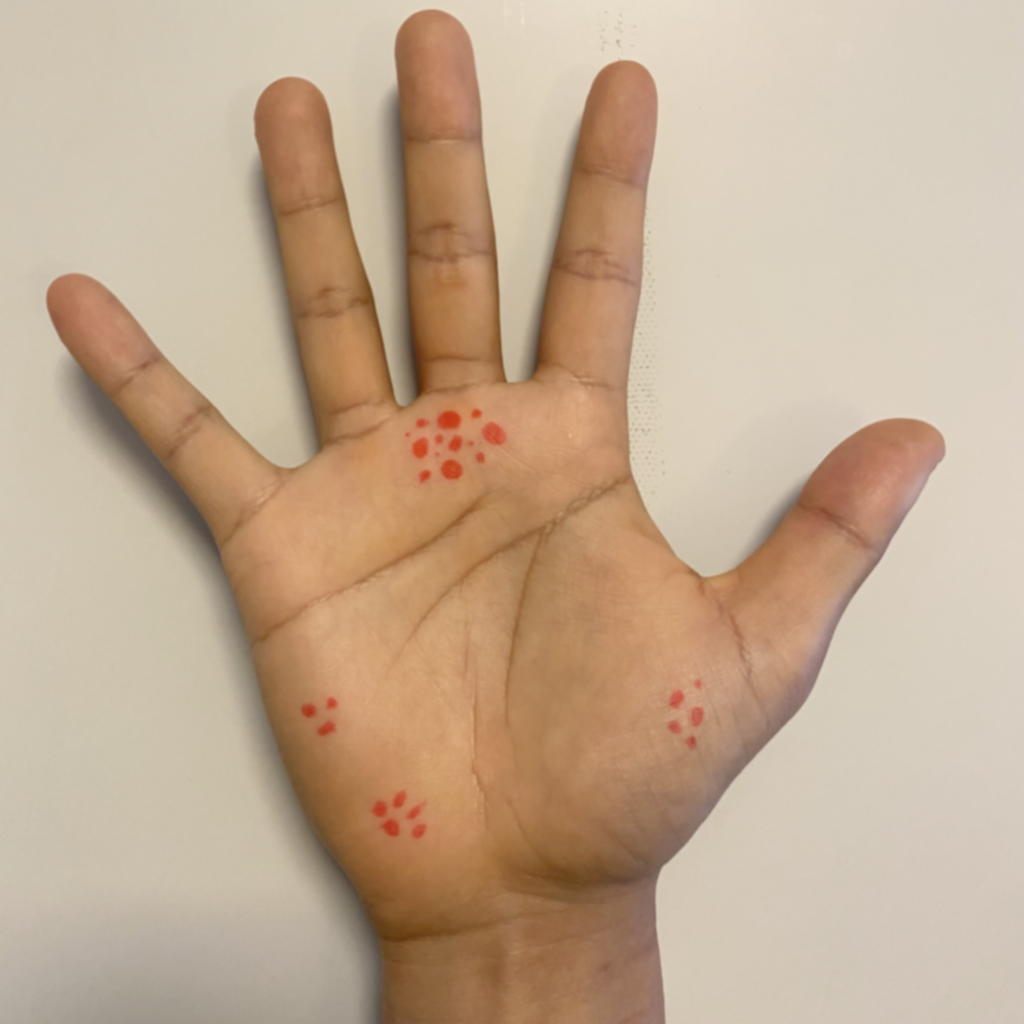
\includegraphics[width=\gridimagewidth,valign=m]{img/supplementary/focus/gaussian_blur/0_gaussian_blur_1.png} & 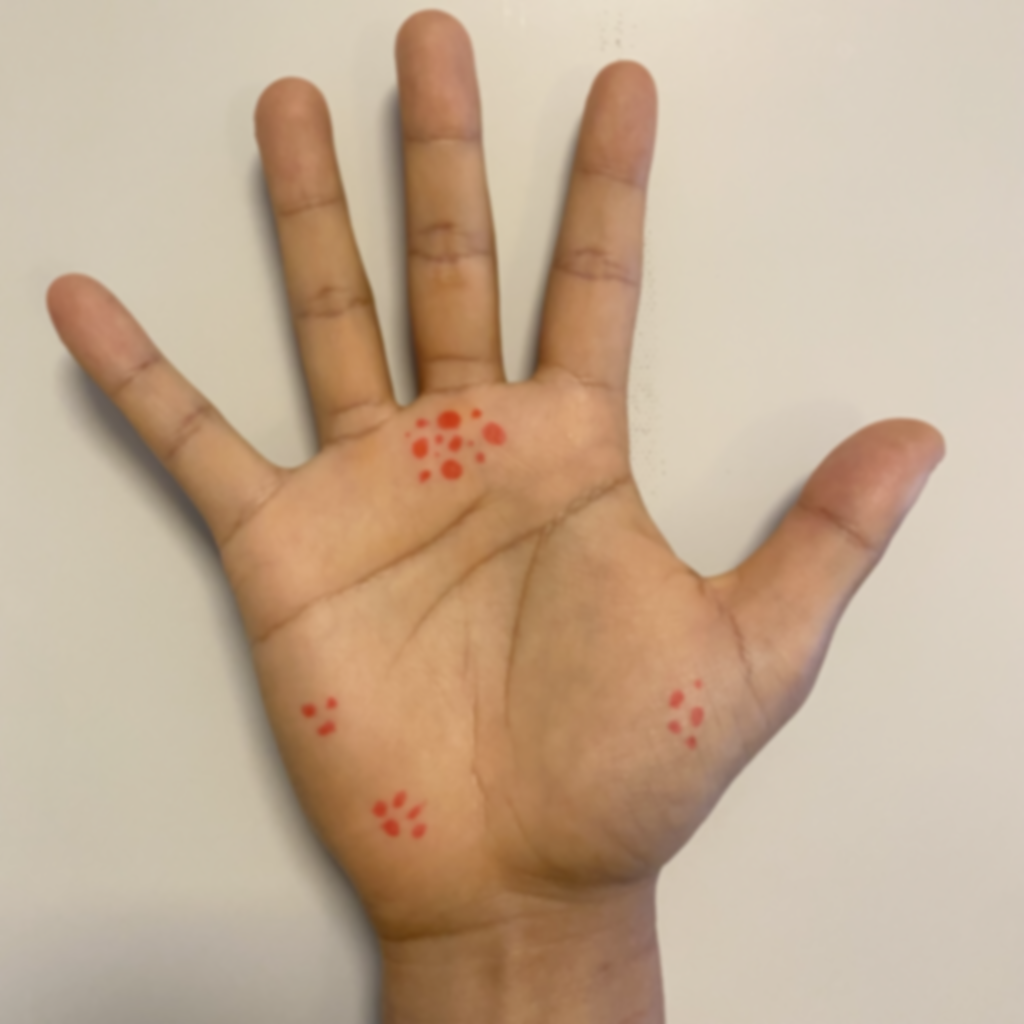
\includegraphics[width=\gridimagewidth,valign=m]{img/supplementary/focus/gaussian_blur/0_gaussian_blur_2.png} & 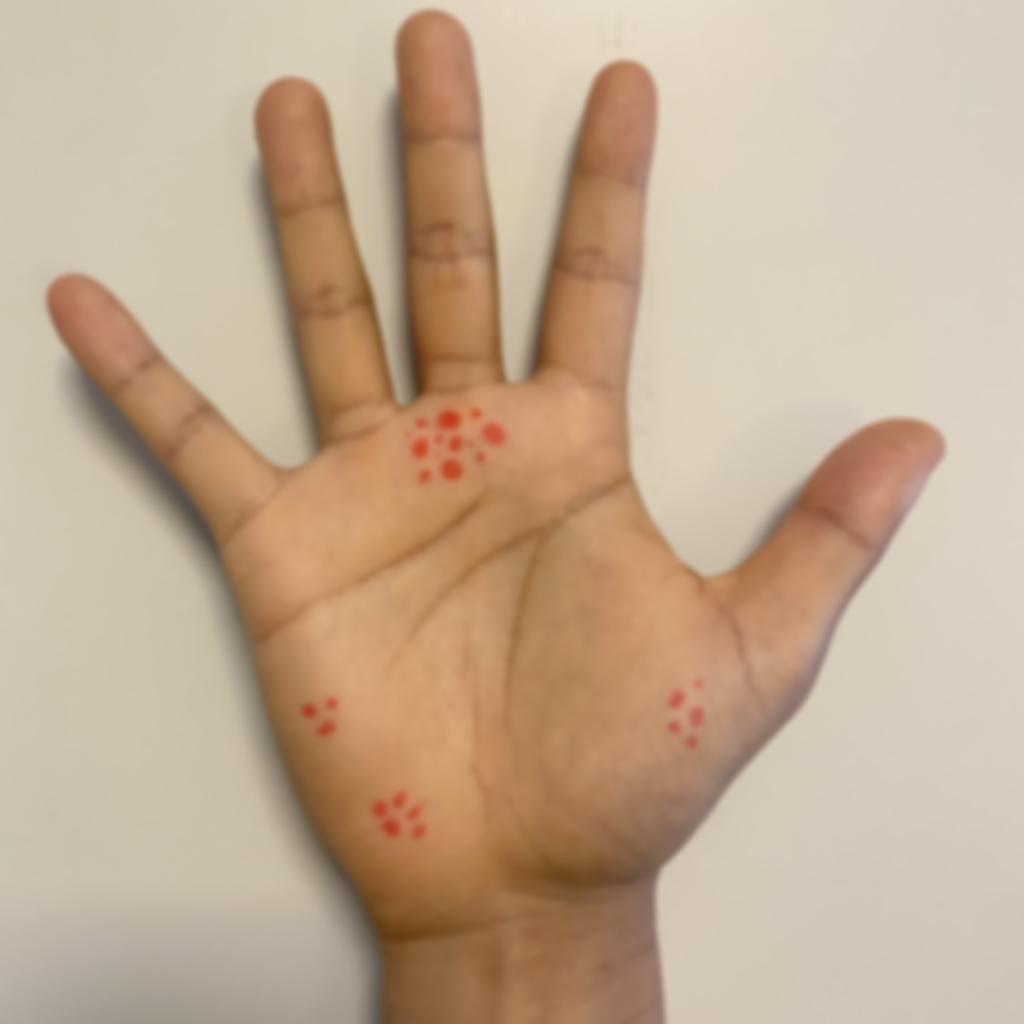
\includegraphics[width=\gridimagewidth,valign=m]{img/supplementary/focus/gaussian_blur/0_gaussian_blur_3.png} & 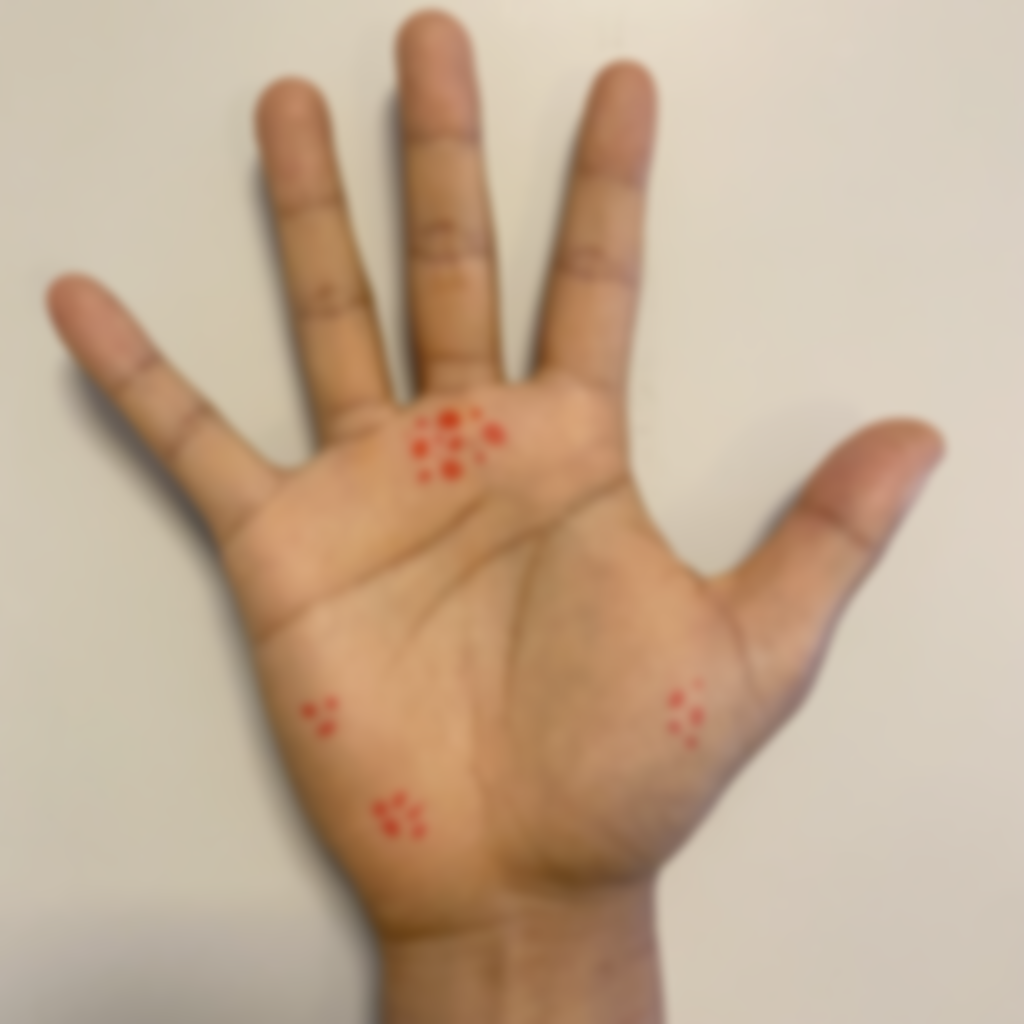
\includegraphics[width=\gridimagewidth,valign=m]{img/supplementary/focus/gaussian_blur/0_gaussian_blur_5.png} \\ [6.15ex]
            Lens blur & 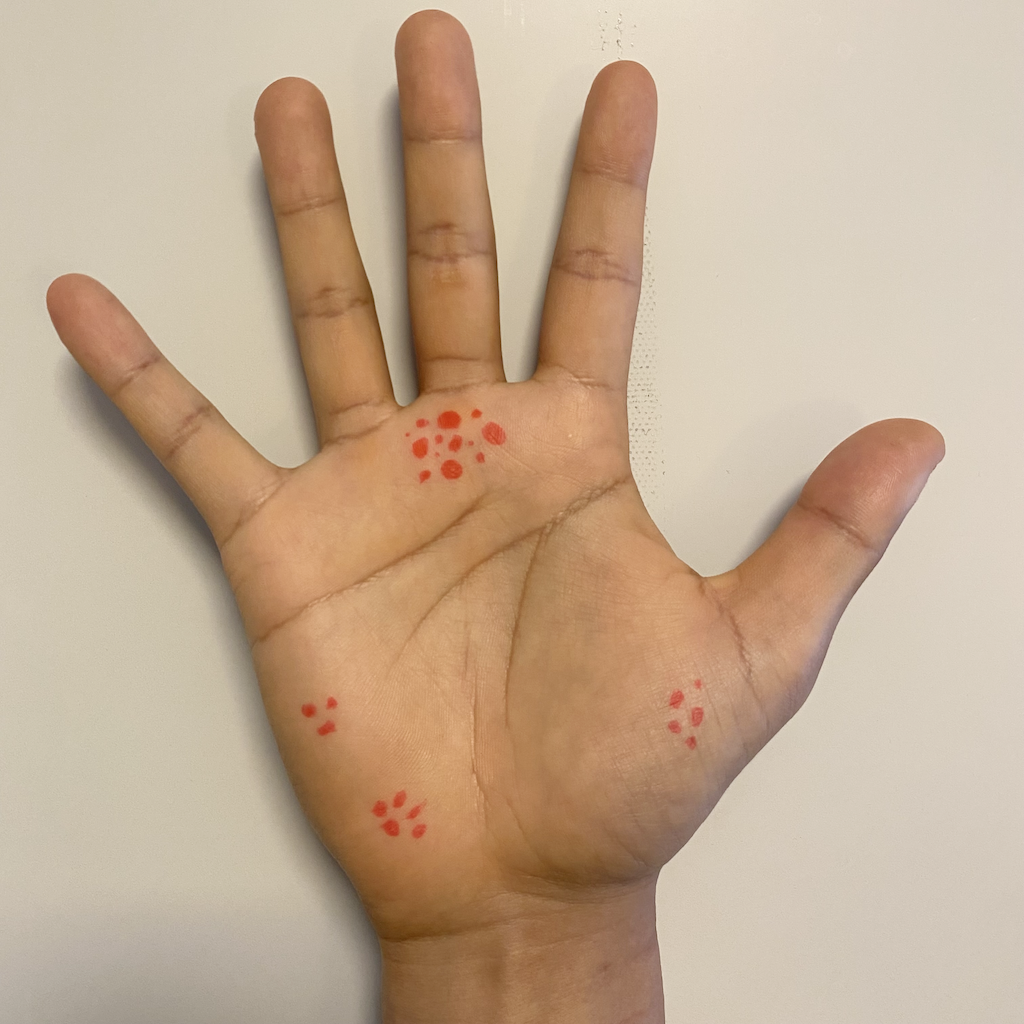
\includegraphics[width=\gridimagewidth,valign=m]{img/supplementary/focus/lens_blur/0_lens_blur_0.png} & 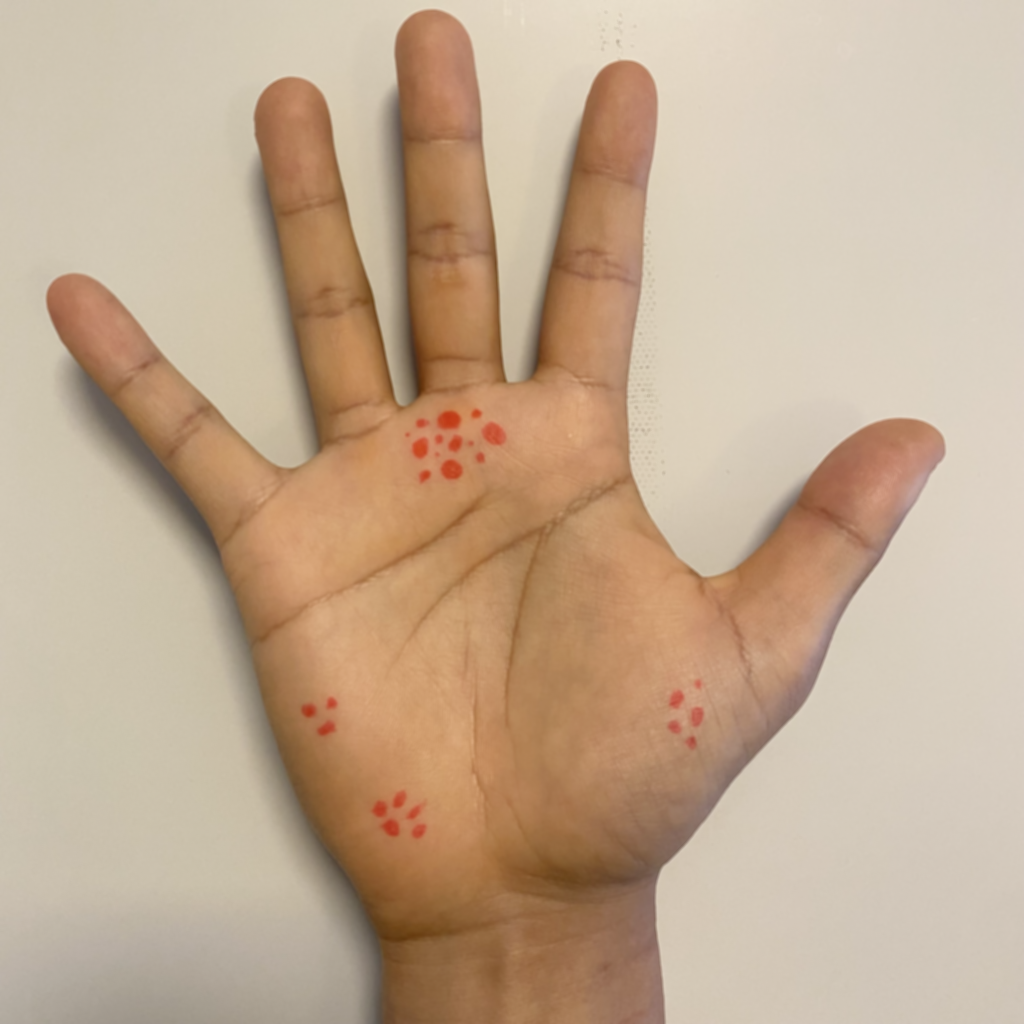
\includegraphics[width=\gridimagewidth,valign=m]{img/supplementary/focus/lens_blur/0_lens_blur_2.png} & 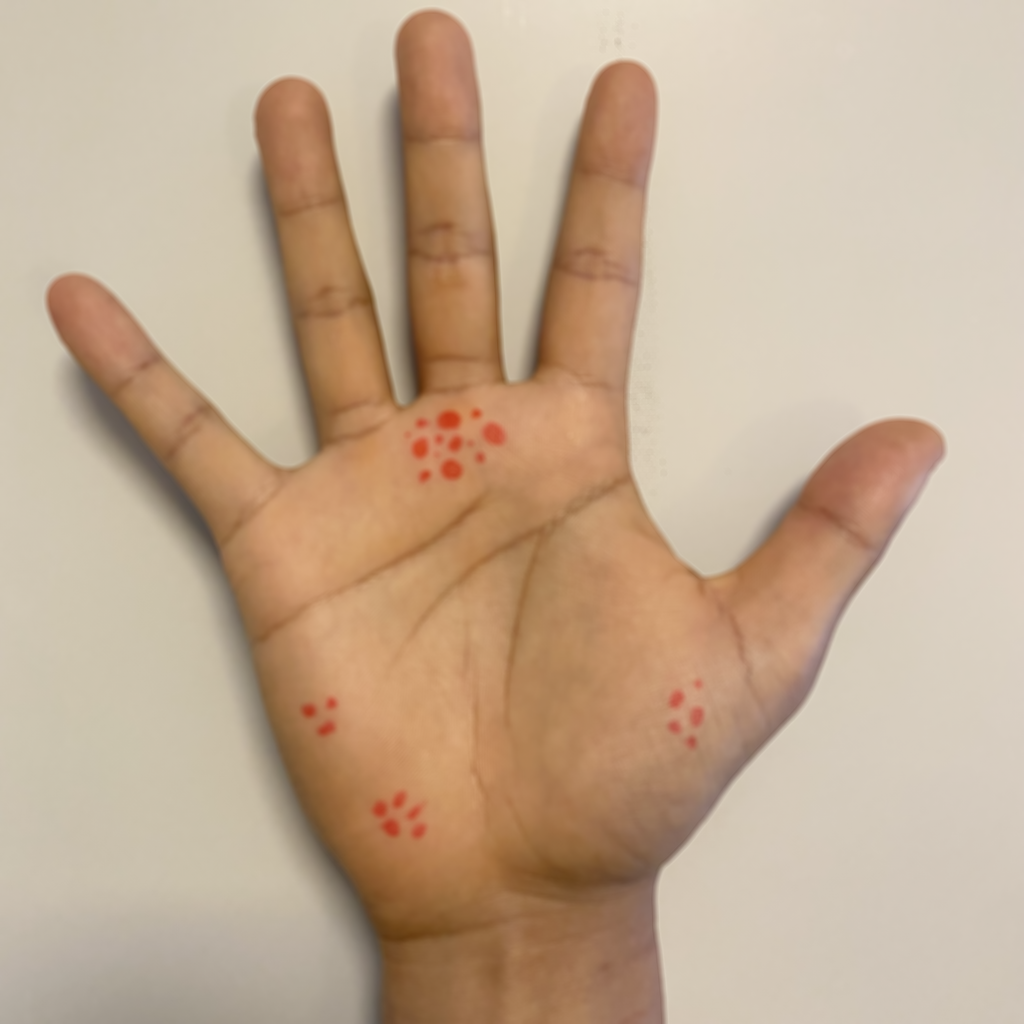
\includegraphics[width=\gridimagewidth,valign=m]{img/supplementary/focus/lens_blur/0_lens_blur_4.png} & 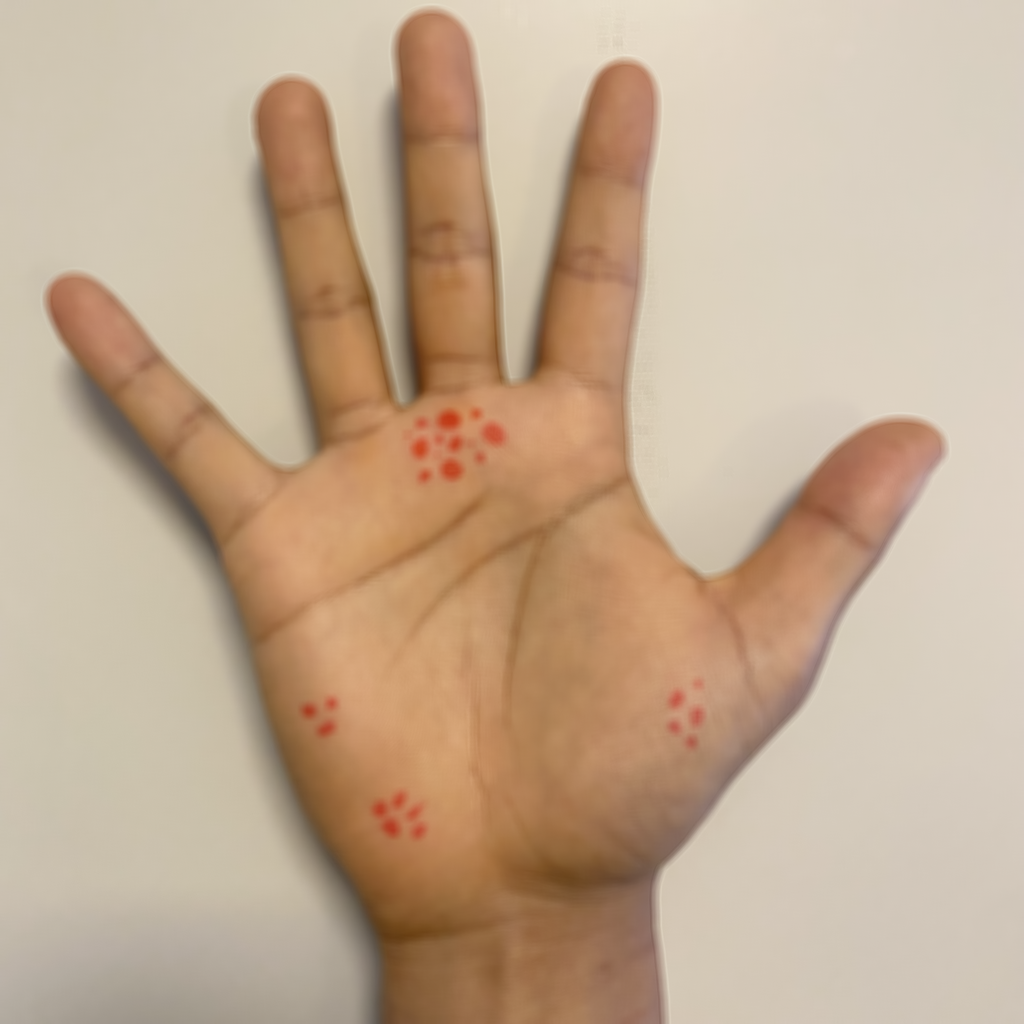
\includegraphics[width=\gridimagewidth,valign=m]{img/supplementary/focus/lens_blur/0_lens_blur_6.png} & \includegraphics[width=\gridimagewidth,valign=m]{img/supplementary/focus/lens_blur/0_lens_blur_8.png} \\ [6.15ex]
            Motion blur & \includegraphics[width=\gridimagewidth,valign=m]{img/supplementary/focus/motion_blur/0_motion_blur_0.png} & \includegraphics[width=\gridimagewidth,valign=m]{img/supplementary/focus/motion_blur/0_motion_blur_2.png} & \includegraphics[width=\gridimagewidth,valign=m]{img/supplementary/focus/motion_blur/0_motion_blur_4.png} & \includegraphics[width=\gridimagewidth,valign=m]{img/supplementary/focus/motion_blur/0_motion_blur_6.png} & \includegraphics[width=\gridimagewidth,valign=m]{img/supplementary/focus/motion_blur/0_motion_blur_8.png} \\ [6.15ex]
        \end{tabular}
    }
    \caption{Visualization of the degradation types belonging to the \textit{Brightness change} group for increasing levels of intensity.}
    \label{fig:focus_supplementary}
\end{figure*}

\begin{figure*}
    \centering
    \setlength{\tabcolsep}{1pt}
    \Large
    \resizebox{\textwidth}{!}{%
        \begin{tabular}{C{5em}ccccc}
            & Level 1 & Level 2 & Level 3 & Level 4 & Level 5 \\
            Change resolution & \includegraphics[width=\gridimagewidth,valign=m]{img/supplementary/resolution/change_resolution/0_change_resolution_0.0.png} & \includegraphics[width=\gridimagewidth,valign=m]{img/supplementary/resolution/change_resolution/0_change_resolution_0.2.png} & \includegraphics[width=\gridimagewidth,valign=m]{img/supplementary/resolution/change_resolution/0_change_resolution_0.4.png} & \includegraphics[width=\gridimagewidth,valign=m]{img/supplementary/resolution/change_resolution/0_change_resolution_0.6.png} & \includegraphics[width=\gridimagewidth,valign=m]{img/supplementary/resolution/change_resolution/0_change_resolution_0.8.png} \\ [6.15ex]
        \end{tabular}
    }
    \caption{Visualization of the degradation types belonging to the \textit{Brightness change} group for increasing levels of intensity.}
    \label{fig:resolution_supplementary}
\end{figure*}

\begin{figure*}
    \centering
    \setlength{\tabcolsep}{1pt}
    \Large
    \resizebox{\textwidth}{!}{%
        \begin{tabular}{C{5em}ccccc}
            & Level 1 & Level 2 & Level 3 & Level 4 & Level 5 \\
            Color saturation 1 & \includegraphics[width=\gridimagewidth,valign=m]{img/supplementary/color_calibration/color_saturation1/0_color_saturation1_0.png} & \includegraphics[width=\gridimagewidth,valign=m]{img/supplementary/color_calibration/color_saturation1/0_color_saturation1_0.2.png} & \includegraphics[width=\gridimagewidth,valign=m]{img/supplementary/color_calibration/color_saturation1/0_color_saturation1_0.4.png} & \includegraphics[width=\gridimagewidth,valign=m]{img/supplementary/color_calibration/color_saturation1/0_color_saturation1_0.6.png} & \includegraphics[width=\gridimagewidth,valign=m]{img/supplementary/color_calibration/color_saturation1/0_color_saturation1_0.8.png} \\ [6.15ex]
            Color saturation 2 & \includegraphics[width=\gridimagewidth,valign=m]{img/supplementary/color_calibration/color_saturation2/0_color_saturation2_0.png} & \includegraphics[width=\gridimagewidth,valign=m]{img/supplementary/color_calibration/color_saturation2/0_color_saturation2_1.png} & \includegraphics[width=\gridimagewidth,valign=m]{img/supplementary/color_calibration/color_saturation2/0_color_saturation2_2.png} & \includegraphics[width=\gridimagewidth,valign=m]{img/supplementary/color_calibration/color_saturation2/0_color_saturation2_3.png} & \includegraphics[width=\gridimagewidth,valign=m]{img/supplementary/color_calibration/color_saturation2/0_color_saturation2_4.png} \\ [6.15ex]
        \end{tabular}
    }
    \caption{Visualization of the degradation types belonging to the \textit{Brightness change} group for increasing levels of intensity.}
    \label{fig:color_calibration_supplementary}
\end{figure*}

\begin{comment}
% Blur
\begin{figure*}
    \centering
    \setlength{\tabcolsep}{1pt}
    \Large
    \resizebox{\textwidth}{!}{ %< auto-adjusts font size to fill line
\begin{tabular}{C{6em}ccccc}
         & Level 1 & Level 2 & Level 3 & Level 4 & Level 5 \\
 Gaussian blur & \includegraphics[width=\gridimagewidth,valign=m]{images/supplementary/distortions/blur/gaublur0.jpg} & \includegraphics[width=\gridimagewidth,valign=m]{images/supplementary/distortions/blur/gaublur1.jpg} & \includegraphics[width=\gridimagewidth,valign=m]{images/supplementary/distortions/blur/gaublur2.jpg} & \includegraphics[width=\gridimagewidth,valign=m]{images/supplementary/distortions/blur/gaublur3.jpg} & \includegraphics[width=\gridimagewidth,valign=m]{images/supplementary/distortions/blur/gaublur4.jpg} \\ [6.15ex]
 Lens blur & \includegraphics[width=\gridimagewidth,valign=m]{images/supplementary/distortions/blur/lensblur0.jpg} & \includegraphics[width=\gridimagewidth,valign=m]{images/supplementary/distortions/blur/lensblur1.jpg} & \includegraphics[width=\gridimagewidth,valign=m]{images/supplementary/distortions/blur/lensblur2.jpg} & \includegraphics[width=\gridimagewidth,valign=m]{images/supplementary/distortions/blur/lensblur3.jpg} & \includegraphics[width=\gridimagewidth,valign=m]{images/supplementary/distortions/blur/lensblur4.jpg} \\ [6.15ex]
 Motion blur & \includegraphics[width=\gridimagewidth,valign=m]{images/supplementary/distortions/blur/motionblur0.jpg} & \includegraphics[width=\gridimagewidth,valign=m]{images/supplementary/distortions/blur/motionblur1.jpg} & \includegraphics[width=\gridimagewidth,valign=m]{images/supplementary/distortions/blur/motionblur2.jpg} & \includegraphics[width=\gridimagewidth,valign=m]{images/supplementary/distortions/blur/motionblur3.jpg} & \includegraphics[width=\gridimagewidth,valign=m]{images/supplementary/distortions/blur/motionblur4.jpg} \\ 
\end{tabular}
}
\caption{Visualization of the degradation types belonging to the \textit{Blur} group for increasing levels of intensity.}
\label{fig:blur_supplementary}
\end{figure*}
\end{comment}


\chapter{Code}
\label{ch:Code}
Anhang, Abkürzungs-, Abbildungs-, Tabellen-, Formel-Verzeichnis, Literaturverzeichnis nicht vergessen!\par
\textbf{Anhänge}

Projektspezifisch können weitere Dokumentationsteile angefügt werden wie:

Aufgabenstellung, Projektmanagement-Plan/Bericht, Testplan/Testbericht, Bedienungsanleitungen, Details zu Umfragen, detaillierte Anforderungslisten, Referenzen auf projektspezifische Daten in externen Entwicklungs- und Datenverwaltungstools etc.
\begin{lstlisting}[caption={Caption on PDF}, label={lst:reference_this}, language=Python]
import numpy as np
\end{lstlisting}